\documentclass[10pt, a4paper]{report}[08.12.2015]
\usepackage[german,ngerman]{babel}
\usepackage[utf8]{inputenc}
\usepackage[T1]{fontenc}
\usepackage{hyperref}
\usepackage[normalem]{ulem}
\usepackage{graphicx}
\usepackage{float}
\usepackage[onehalfspacing]{setspace}
\usepackage{numprint}
\setlength{\parindent}{0pt}
\newcommand\invisiblechapter[1]{%
  \refstepcounter{chapter}%
  \addcontentsline{toc}{chapter}{\protect\numberline{\thechapter}#1}%
  \sectionmark{#1}}


%\setkomafont{section}{\Large\linespread{1}\sffamily}

\begin{document}
  \begin{titlepage}
	\centering
	
\includegraphics[width=0.25\textwidth]{secondlogo.png}\par\vspace{1cm}
	{\scshape\LARGE Zentrum f\"ur Bioinformatik (ZBH)\par}
	{\scshape\LARGE Universit\"at Hamburg \par}
	{\scshape\LARGE Hamburg, Deutschland \par}
	\vspace{1cm}
	{\scshape\Large Projekt Genominformatik\par}
	\vspace{1.5cm}
	{\huge\bfseries Ein systematischer Vergleich von Verfahren zur 					funktionellen und taxonomischen Klassifikation von metagenomischen 				Sequenzfragmenten\par}
	\vspace{2cm}
	{\Large\itshape Marie-Sophie Briem, Inga Lemme, Sarah Weber\par}
	\vfill
	Gutachter/in\par
	Prof. Dr.~Kurtz, Dr. Gonella 

	\vfill

% Bottom of the page
	{\large \today\par}
\end{titlepage}

  \pagenumbering{roman}
  \newpage
  \tableofcontents
  \newpage
  \listoffigures
  \newpage
  \pagenumbering{arabic}
   \chapter{Einleitung}
    Der Forschungsbereich der Metagenomik besch\"aftigt sich mit der Klassifizierung und Zuordnung aller genetischen Informationen, die in zuf"allig entnommenen Proben enthalten sind \cite{handelsman1998}. Die Proben bestehen beispielsweise aus marinen mikrobiellen Wasser- oder Bodenproben, mit Hilfe derer \"okologische Fragestellungen beantwortet werden sollen. Ein weiteres bedeutsames Forschungsgebiet der Metagenomik ist die Besch\"aftigung mit dem humanen Mikrogenom welches wichtige Informationen unter anderem zur Ern\"ahrung, Regulation des Immunsystem und der Aufkl\"arung von Krankheitsresistenzen geben kann \cite{dethlefsen2008}. Aus diesen Proben wird die gesamte enthaltene DNA extrahiert und sequenziert. Anschlie{\ss}end werden die Proteine annotiert um Funktion und taxonomische Zuordnung der enthaltenden Spezies zu ermitteln (Abb. \ref{fig:metagenom}).
    Basierend auf neuen und schnellen Sequenzierungstechnologien wie Illumina, fallen im Bereich der Metagenomik gro{\ss}e Datenmengen an, die taxonomisch und funktionell klassifiziert werden m\"ussen. Eine vielversprechende Alternative zu dem Alignierprogramm BlastX, welches mithilfe von Sequenzvergleichen eine solche Klassifizierung durchf\"uhrt, scheinen Diamond \cite{buchfink2014} und Lambda \cite{hauswedell2014} zu sein, die eine Laufzeitersparnis mit Hilfe von double indexing erwirken sollen.
    \newline
    \begin{figure}[H]
\centering
      \noindent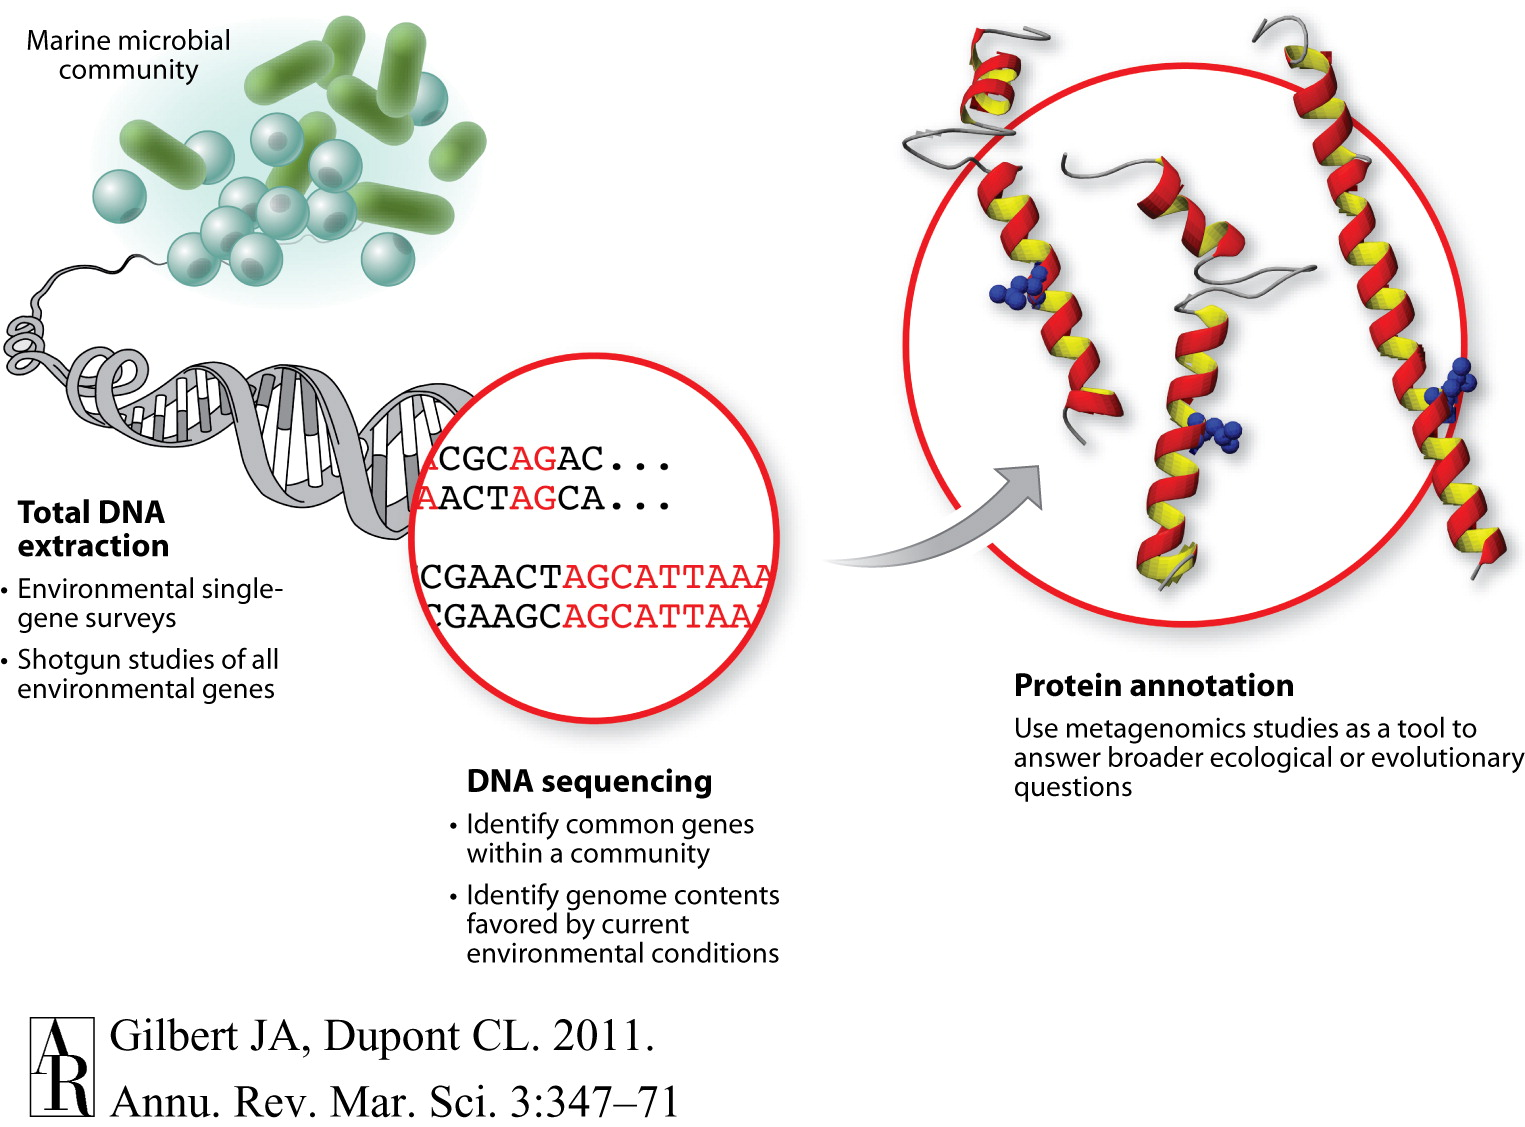
\includegraphics[width=\linewidth,height=15cm,
      keepaspectratio]{Abbildungen/metagenome-steps.jpg}
      \caption{Metagenomik in Schritten}
      \label{fig:metagenom}
\end{figure}
   
   \section{\textrm{Lambda}}
   Das open source verf\"ugbare Alignierprogramm Lambda \cite{hauswedell2014} basiert auf einem Seed- und Extent Algorithmus. Im Gegensatz zu Diamond muss die Refernzdatenbank vorab indiziert werden und findet nicht w\"ahrend des Programmdurchlaufs statt. Als Datenstrukturen stehen f\"ur die Referenzdatenbank ein Suffixarray und f\"ur die Anfragesequenz ein Radixtree zur Verf\"ugung. Die Speicherung in einem Radixtree erm\"oglicht eine Paralellisierung verschiedener Seeds, was eine zus\"atzliche Zeitersparnis bedeutet. 
    Die Erweiterung erflolgt mit Hilfe des X-drop Algorithmus. 
    
    \section{\textrm{Diamond}}    
     Auch Diamond \cite{buchfink2014} basiert wie Lambda auf dem Seed- und Extend Algorithmus mit Double Indexing. Im Seedingschritt werden so gennante Spaced Seeds gesucht, die als Treffer in Anfrage- und Datenbanksequenz gefunden werden sollen (Abb.  \ref{fig:diamond}). Das Seeding findet anschlie{\ss}end mit Double Indexing statt. Beim Double Indexing werden sowohl Anfrage- als auch Referenzdatenbanksequenz geindext, was eine geringere Laufzeit durch schnelleres durchsuchen der Datenstrukturen mit sich bringt. Die Indizierung findet bei Diamond $"$on the fly$"$, das hei{\ss}t w\"ahrend des Programmdurchlaufs, statt. Die Treffer, die mit Hilfe der Spaced Seeds gefunden wurden, speichert Diamond in lexikographisch sortierten Listen.
\begin{figure}[h]
\centering
      \noindent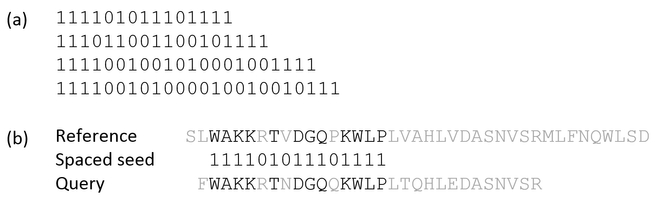
\includegraphics[width=\linewidth,height=15cm,
      keepaspectratio]{Abbildungen/diamond_spacedSeeds.jpg}
      \caption{Spaced Seeds}
      \label{fig:diamond}
\end{figure}
\newline
    Um eine Erweiterung im Extendschritt durchzuf\"uhren, \"uberpr\"uft das Programm, ob der Seed-Treffer gr\"o{\ss}er-gleich 10 Aminos\"auren lang ist. Der Seed wird schlie{\ss}lich mit dem Smith-Waterman Algorithmus erweitert.
\newline
    
    
 
    \section{Ziele}
    
    Das Projekt hat folgende Ziele:
    
    \begin{itemize}
    
      \item Bestimmung und Vergleich der Sensivit"at (Anzahl an korrekt Bestimmten / Anzahl an Sequenzen im Datenset) und Pr\"azision (Anzahl an korrekt Bestimmten / Anzahl an Zugewiesenen) der Programme \textrm{Diamond} 				und \textrm{Lambda}.
      
      \item Bestimmung und Vergleich der ben"otigten Zeit der Programme
      		\textrm{Diamond} und \textrm{Lambda}.

      
    
    \end{itemize}


    \newpage
  \chapter{Material und Methoden}
    
    \section{Material} 
    
      Das durchgef"uhrte Projekt orientiert sich an der Forschungsarbeit von
      Bazinet und Cummings \cite{bazinet2012}. Im 
      Folgenden bezieht sich der Ausdruck $"$Vorlagepaper$"$ auf die Arbeit von
      Bazinet und Cumming. Die Datensets und Datenbanken wurden anhand des 			  Vorlagepapers ausgew"ahlt.
      
      \subsection{Benchmark-Datens"atze}
      \label{subsec:Datens"atze}
        Die Experimente wurden mit folgenden Benchmark-Datens"atzen 					durchgef"uhrt:
        
        \begin{enumerate}
        
          \item \textit{FACS 269bp} $-$ Datensatz, original von Strannenheim 			  \textit{et al.} \cite{stranneheim2010}, bestehend aus
          \textbf{\numprint{27049} simulierten 454 
          Reads} mit einer durschnittlichen L"ange von \textbf{269 bp}. Die
          im $"$Vorlagepaper$"$ angegebene Referenz war nicht mehr aktuell 				  und konnte nicht gefunden werden. Der Datensatz wurde direkt von 				  Herrn Bazinet bereit gestellt. Der bereitgestellte Datensatz 					  beinhaltet \numprint{72951} Reads der Spezies \textit{Homo sapiens}. Diese 				  Reads wurden entfernt, so dass der genutzte Datensatz \numprint{27049} Reads 			  enth\"alt. Der Datensatz setzt sich aus 19 bakteriellen und drei 				  viralen Genomen zusammen \cite{bazinet2012}.  
           
          \item \textit{CARMA 265bp} $-$ Datensatz bestehend aus
          \textbf{\numprint{25000} simulierten 454 Reads} mit einer durschnittlichen 				  L"ange von \textbf{265 bp}, original genutzt von Gerlach und Stoye
          \cite{GerlachStoye2011}. Der Datensatz wurde von der WebCARMA 				  Homepage unter dem Link \url{http://wwww.cebitec.uni-							  bielefeld.de/webcarma.cebitec.uni-											  bielefeld.de/download/simulated_metagenome_454_265bp.fna}
          heruntergeladen. Zusammengesetzt ist der Datensatz aus 25 				 	  bakteriellen Genomen, die sich wie folgt in die einzelnen 					  bakteriellen Phyla verteilen: 73,0\% Proteobacteria; 12,9\% 					  Firmicutes; 7,8\% Cyanobacteria; 5,2\% Actinobacteria; 1,0\% 					  Clamydiae \cite{bazinet2012}.
          
          \item \textit{Metaphyler 300bp} $-$ Datensatz bestehend aus 
          \textbf{\numprint{73086} simulierten
          Reads} von 31 phylogenetischen Markern bakterieller Genome mit 			  	  einer durschnittlichen L"ange von \textbf{300 bp}. Urspr\"unglich 			  genutzt von Liu \textit{et al.} \cite{Liu2010}. Der
          Datensatz konnte anhand der im $"$Vorlagepaper$"$ angegebenen 				  Referenz nicht korrekt ermittelt werden. Die Rechercheergebnisse
          ergaben einen Datensatz bestehend aus \numprint{40039} Reads mit einer 
          durchschnittlichen L"ange von 645 bp. Der korrekte
          Datensatz wurde direkt von Herrn Bazinet bereit gestellt. 
          Die Verteilung in die bakteriellen Phyla setzt sich folgenderma"sen 		  zusammen: 47.0\% Proteobacteria; 21.9\% Firmicutes; 9.7\% 					  Actinobacteria; 4.8\% Bacteroidetes; 3.9\% Cyanobacteria; 2.2\% 				  Tenericutes; 1.9\% Spirochaetes; 1.3\% Chlamydiae; 0.9\% 						  Thermotogae; 0.9\% Chlorobi \cite{bazinet2012}. 
          
          \item \textit{PhymmBL 243bp} $-$ Datensatz bestehend aus 
          \textbf{\numprint{80215} RefSeq
          Reads} mit einer durschnittlichen L"ange von
          \textbf{243 bp}. Der Datensatz, original genutzt von Brady und 
          Salzberg \cite{bradysalzberg2009},  
          konnte anhand der im $"$Vorlagepaper$"$ angegebenen Referenz nicht 
          korrekt ermittelt werden. Die Rechercheergebnisse
          ergaben einen Datensatz bestehend aus \numprint{73252} Reads mit einer 
          durchschnittlichen L"ange von 204 bp. Der korrekte
          Datensatz wurde direkt von Herrn
          Bazinet bereit gestellt.  
          
          \item \textit{PhyloPythia 969bp} $-$ simMC Datensatz bestehend aus
          \textbf{\numprint{114457} Reads} mit einer durschnittlichen L"ange von
          \textbf{969 bp}, original von Patil \textit{et al.} 							  \cite{patil2011}. Der im $"$Vorlagepaper$"$ verwendete Datensatz 
          "PhyloPythia"\ bestehend aus \numprint{124941} Reads mit einer 
          durchschnittlichen L"ange von 961 bp konnte
          auch mit Hilfe von Herrn Bazinet nicht ermittelt werden.
          Der Datensatz wurde von der JGI Homepage unter dem Link
          \url{http://fames.jgi-psf.org/Retrieve_data.html} heruntergeladen.  
          
          \item \textit{RAIphy 233bp} $-$ Datensatz bestehend aus
          \textbf{\numprint{477000} RefSeq Reads} mit einer durschnittlichen L"ange von
          \textbf{233 bp}, original von Nalbantoglu \textit{et al.} 					  \cite{nalbantoglu2011}. Der im $"$Vorlagepaper$"$ verwendete 					  Datensatz "RAIphy"\ bestehend aus \numprint{477000} Reads mit einer 
          durchschnittlichen L"ange von 238 bp konnte
          mit der angegebenen Referenz und auch mit Hilfe von Herrn Bazinet 			  nicht ermittelt werden. Der im Projekt verwendete Datensatz wurde 			  von Herrn Bazinet zur Verf"ugung gestellt.
          
        \end{enumerate}
        
      \subsection{Datenbank}
      F\"ur die Suche wurde die Datenbank UniProtKB/Swiss-Prot von UniProt 			  verwendet \cite{bairoch2004}.
      Diese wurde unter dem Link \url{http://www.uniprot.org/downloads}
      heruntergeladen.
      Die Datenbank besteht aus \numprint{549646} Sequenzen mit einer 						  durchschnittlichen L\"ange von \numprint{35656}bp.
      \subsection{Programme}
      \label{subsec:Programme}
        Im Projekt wurden folgende Programme verwendet:
        
        \begin{enumerate}
          
          \item \textbf{Lambda} $-$ Das Programm Lambda (Version 0.9.2) \cite{hauswedell2014} wurde 			  von der GitHub Seite mit dem Link 											  \url{https://github.com/seqan/lambda.git} heruntergeladen 					  . Dabei wurde wie folgt vorgegangen:
          \begin{itemize}
            \item[\$] git clone \url{https://github.com/seqan/lambda.git}
            \item[\$] cd lambda
            \item[\$] mkdir build
            \item[\$] cmake																    -DCMAKE\_C\_COMPILER=/usr/local/zbhtools/gcc/gcc-5.1.0/bin/gcc 
            -DCMAKE\_CXX\_COMPILER=/usr/local/zbhtools/gcc/gcc-5.1.0/bin/g++ 
            -DCMAKE\_INSTALL\_PREFIX=\$/work/gi/software 
            \item[\$] make -j2													   
          \end{itemize}
          Um das Programm Lambda ausf\"uhren zu k\"onnen musste die 					  UniProtKB/Swiss-Prot Datenbank zun\"achst indiziert werden. Dazu 				  wurde das Programm "lambda\_indexer"\ verwendet, welches in dem 				  oben genannten Packet enthalten ist. Folgender Aufruf wurde 					  verwendet:
          \begin{itemize}
            \item[\$] lambda\_indexer -d uniprot\_sprot.fasta
          \end{itemize}
          Die jeweiligen Datensets (s.o.) wurden gegen die indizierte 					  Datenbank mit dem Befehl
          \begin{itemize}
            \item[\$] lambda -q QUERY.fasta -d DATABASE.fasta [-o output.m8]
          \end{itemize}
          aligniert.
          
          
          \item \textbf{Diamond} $-$ Das Programm Diamond (Version 0.7.9) 				  \cite{buchfink2014} wurde 
          von der GitHub Seite mit dem Link
          \url{https://github.com/bbuchfink/diamond.git} heruntergeladen
          . Es wurde folgenderma\ss{en} verfahren:
          \begin{itemize}
            \item[\$] git clone 															\url{https://github.com/bbuchfink/diamond.git}
            \item[\$] cd diamond
            \item[\$] mkdir build
            \item[\$] cmake 																-DCMAKE\_INSTALL\_PREFIX=\$/work/gi/software/diamond
            \item[\$] make install
		  \end{itemize}
		  Mit dem Aufruf
		  \begin{itemize}
		    \item[\$] diamond makedb --in uniprot\_sprot.fasta -d 							diamonduniprot\_sprot.fasta.dmnd
		  \end{itemize}
		  wurde die bin\"are Diamond-Datenbank aus der UniProtKB/Swiss-Prot
		  Datenbank erstellt.\newline
		  Die jeweiligen Datensets (s.o.) wurden gegen die zuvor erstellte 				  Diamond-Datenbank mit dem Befehl
		  \begin{itemize}
		    \item[\$] diamond blastx -d DIAMOND\_DATABASE.dmnd -q QUERY.fasta 			-a OUTPUT -t <temporary directory> 
		  \end{itemize}
		  aligniert.		             
          
          \item \textbf{MEGAN5} $-$ Das Programm MEGAN5 (Version 5.10.7) 				  \cite{huson2011} wurde von der Website \url{http://ab.inf.uni-									  tuebingen.de/data/software/megan5/download/welcome.html}
          heruntergeladen . Die ben\"otigte akademische
          Lizenz wurde von Herrn Dr. Gonella zur Verf\"ugung 
          gestellt. MEGAN5 ist ein Programm mit einer graphischen 						  Benutzeroberfl\"ache. Das Programm ben\"otigt eine "map"\ gegen die
          es die Eingabereads vergleicht. Es konnte nicht die 				  		  voreingestellte "map"\ genutzt werden, da diese gegen genomspezifische Identifikationsnummern sucht, die Ausgabe von Lambda und Diamond jedoch durch die Nutzung der UniProtKB/Swiss-Prot Datenbank sp-Nummern generiert. Aus diesem Grund wurde die $"$idmapping.dat"\ 				  von der Website 									\url{ftp://ftp.uniprot.org/pub/databases/uniprot/current_release/knowledgebase/idmapping/} 		  heruntergeladen. Diese wurde anschlie{\ss}end gek\"urzt, so dass 				  nur die Taxa enthalten waren, die auch in der UniProtKB/Swiss-Prot 			  Datenbank vorkommen. 
          
          
            \item \textbf{Newick-Parser} $-$ Das Programm $"$newick-parse$"$ 
            wurde von Prof. Dr. Kurtz zur Verf"ugung gestellt und ist 
            Teil des Taxtree-Packets \cite{kurtz2016}. F"ur die Berechnung der Distanzen
            zwischen dem Gold-Standard und den von MEGAN5 ermittelten Taxa
            wurde folgender Aufruf verwendet:
			\begin{itemize}
			  \item[\$] ruby newick-parse.rb $--$lca samples.txt $--$path-					  length all\_ids.tre
		    \end{itemize}			            
            
        \end{enumerate}
        \newpage
    \section{Methoden}
    
       \subsection{Vorarbeit}
        Bevor die Ausgaben mit den Programmen Diamond und Lambda erzeugt werden konnten, mussten einige Schritte im Vorfeld durchgef"urht werden. Zun"achst wurden mithilfe des $"$Vorlagepaper$"$ \cite{bazinet2012} die zu verwendenden Benchmark-Datens"atze ausgew"ahlt ( \ref{subsec:Datens"atze} ). Einige Benchmark-Datens"atze waren auf mehrere Fasta-Dateien aufgeteilt worden. Da die Programme Diamond und Lambda in ihrem Aufruf nur eine Anfragesequenzdatei erlauben, wurden die zu einem Benchmark-Datensatz geh"origen Fasta-Dateien zu einer konkatiniert. \newline
      Die Benchmark-Datens"atze enthalten zum Teil komplette Genome einer Spezies, die in mehrere Reads aufgeteilt wurden. Die Header-Zeilen dieser Reads enthalten alle die gleichen Identifikationsnummern, da diese lediglich Auskunft "uber die Spezies und nicht "uber den Genomabschnitt geben. Damit jedes Genom-Fragment in der Auswertung ber"ucksichtigt werden konnte, wurden alle Header-Zeilen mit einer Read-Id aufsteigend nummeriert. \newline
      Bei den ersten Probe-Durchl"aufen mit Lambda und Diamond fielen noch zwei weitere Schwierigkeiten auf. Zum einen enthielt der Benchmark-Datensatz FACS mehrere Humangenome, welche nicht in die Auswertung eingehen sollten, weshalb dieses entfernt wurde. Zum anderen ergab sich ein Problem beim Generieren einer Lambda-Ausgabe mit dem Benchmark-Datensatz PhyloPythia. Als Wildcard-Symbol enthielt dieser ein 'X', welches von Lambda nicht ausgewertet werden konnte. Aus diesem Grund wurde dieses durch ein 'N' ersetzt.

      \subsection{Programmausgabe}
      Die Ausgaben f"ur Lambda und Diamond wurden mit allen Benchmark-Datens"atzen wie in \ref{subsec:Programme} beschrieben, generiert.
      
            \subsection{Taxonomische Zuordnung}
      In den Programmausgaben wurde ein Read aus den Benchmark-Datens"atzen zu mehreren Reads der Referenzdatenbank zugeordnet. Um eine eindeutige taxonomische Zuordnung zu erhalten, wurde das Programm MEGAN5 verwendet, welches zu einem Read aus dem Benchmark-Datensatz den lowest common ancestor (LCA) in der Referenz-Datenbank sucht und den mit dem kleinsten LCA zuordnet. Au{\ss}erdem wird die Id aus der Datenbank, die als eine sp-Nummer repr"asentiert ist, durch eine NCBI Taxid ersetzt. Einige Reads aus den Benchmark-Datens"atzen konnten von MEGAN5 nicht zugeordnet werden. \newline \newline
      Um anschlie{\ss}end "uberpr"ufen zu k"onnen, wie exakt die Zuordnungen der Programme Lambda und Diamond waren, wurde ein sogenannter Gold-Standard erstellt, der den Benchmark-Datens"atzen die tats"achlichen Taxids zuordnet. F"ur die Erstellung des Gold-Standard wurde die map $"$gi\_taxid\_nucl.dmp$"$ von der Website  \url{ftp://ftp.ncbi.nih.gov/pub/taxonomy/} verwendet.
      
      \subsection{Genauigkeitsberechnungen}
             \label{subsec:Genauigkeitsberechnungen}

      Mit Hilfe des $"$newick-parse$"$ wurde schlie{\ss}lich der LCA zweier Taxids berechnet, die in der Megan-Ausgabe und im Gold-Standard zum gleiche Read zugeordnet wurden und die Distanzen vom LCA zu den beiden Taxids addiert. Zur Auswertung der Ergebnisse wurden die Sensitivit"at- und Pr"azisionswerte der Programme Lambda und Diamond mit jedem Benchmark-Datensatz ermittelt.
      \begin{itemize}
      \item[] Sensitivit"at = Anzahl korrekter Reads / Anzahl aller Reads
      \item[] Pr"azision = Anzahl korrekter Reads / Anzahl zugewiesener Reads
      \end{itemize}
      F"ur die Anzahl der korrekten Reads wurden eine Distanz von bis zu f"unf erlaubt und jeweils Sensitivit"at und Pr"azisionen von Distanzen zwischen null und f"unf berechnet. 
      
  \subsection{Meta-Programm}
  Damit die Analyse der Datens"atze schnell vonstatten gehen sollte, wurde ein Meta-Programm in RubyCode geschrieben, dass alle einzelnen Schritte der Analyse beinhalten sollte. Es sollte ebenfalls automatisch ablaufen.
  
  
  Die ersten Schritte, wie die Erstellung eines Programmoutputs der Alignmenterstellung von Lambda und Diamond, sowie die Ausgabe der LCA's von MEGAN mussten manuell gefertigt werden.
  
  Das Meta-Programm beginnt mit dem extrahieren der Readnummern und der Identifikationsnummer aus den Fasta-Dateien. 
  Die Readnummer oder auch Read-Id wird ben"otigt, da diese von den Programmen Lambda, Diamond und Megan als Identifikatoren der einzelnen Reads "ubernommen wird.
  
 Die Identifikationsnummer wird ben"otigt um mit Hilfe von maps f"ur bestimmte Identifikationsnummern, zum Beispiel gi-Nummer, deren passende taxonomie Indetifikatoren zu erhalten.
  Also wurde nach den Schritt der Extraktion von Read-Id und ID, die passende taxonomische map durchsucht um f"ur jeden Read die passende Tax-Id zu erhalten.
  Das ist dann in diesem Fall der Gold-Standart.
  Der folgende Schritt bezieht sich auf den Vergleich von dem Gold-Standard f"ur einen Read zur Tax-Id, die von Megan ausgegeben wurde. Daf"ur wurde vom Meta-Programm eine tempor"are Datei erstellt, die die Gold-Tax-Id neben die Megan-Tax-Id aufstellt, seperiert durch einen Tab. Diese Datei wurde dann von dem $"$newick-parse$"$ ausgelesen und erstellte einen Output mit den Pfadunterschieden der beiden Taxa. Das heisst, f"ur jeden Read, der von Lambda und Diamond einer oder mehreren Referenzsequenz$/$en zugeordnet wurde, wurde der Pfadunterschied von der Megan-Tax-Id hin zu der des Gold-Standards aufgezeigt.
  Diese Pfadunterschiede wurden anschliessend analysiert. 
  Der letzte Schritt des Meta-Programms ist die Berechnung der Sensitivit"at sowie die Pr"azision \ref{subsec:Genauigkeitsberechnungen}.
  Diese werden f"ur jeden Datensatz in einer Datei ausgegeben. In der Datei befindet sich auch die Auflistung mit der H"aufigkeit der Distanzen zwischen Gold-Standard und der Meganasugabe. 
  
  Die H"aufigkeitsverteilung wurde anschliessend manuell f"ur die Erstellung der Histaogramms verwendet.  
  
  
    \newpage
  \chapter{Ergebnisse}
    \section{Distanzverteilung}
    \label{sec:distanzverteilung}
  Die Histogramme, welche die Distanzverteilungen abbilden, sind im Anhang zu finden. Die Abbildungen  \ref{fig:carma} - \ref{fig:raiphy}  zeigen die Distanzverteilungen der Reads, welche mithilfe des newick-parser ermittelt wurden. Um einen direkten Vergleich von Diamond und Lambda vornehmen zu k\"onnen, wurden pro Benchmark-Datensatz die Ergebnisse beider Programme gegeneinander gestellt.
  \newline
   Die Verteilungen der Benchmark-Datens\"atze Carma (Abb. \ref{fig:carma}), FACS (Abb. \ref{fig:facs}) und PhyloPythia (Abb. \ref{fig:phylopythia}) zeigen die gemeinsame Tendenz, dass das Programm Diamond eine hohe Anzahl an Zuweisungen vornimmt, die eine geringe Distanz zu den 
  tats"achlichen Taxa aufweisen. Die Ausgaben von Lambda zeigen erst bei einer Distanzgr\"o{\ss}e von gr\"o{\ss}er als 4 bemerkenswerte Readanzahlen.
  \newline
    Die jeweiligen Ergebnisse der beiden Programme f\"ur die \"ubrigen drei 		Datens\"atze (Abb. \ref{fig:metaphyler} - \ref{fig:raiphy}) \"ahneln sich sehr. Auff\"allig ist hier, dass
    die Zuweisung der Reads bei beiden Programmen f\"ur die Datens\"atze 			Metaphyler (Abb. \ref{fig:metaphyler}) und PhymmBL (Abb. \ref{fig:phymmbl}) erst nennenswerte Readanzahlen 		bei einer Distanz von gr\"o{\ss}er als 4 erzeugen. F\"ur den Benchmark-Datensatz
    RAIphy k\"onnen bei beiden Programmen hohe Readanzahlen bei einer Distanz
    von 0 beobachtet werden.    \newline
    F\"ur alle Datens\"atze l\"asst sich erkennen, dass Lambda insgesamt 
    mehr Reads zugeordnet hat als Diamond.
  
     \section{Sensitivit"at und Pr"azision}
       Die oben beschriebene Tendenz (\ref{sec:distanzverteilung}) zeigt sich auch f"ur die Genauigkeitsberechnungen. Die ausgewertete Lambda-Ausgabe zeigt f"ur den Benchmark-Datensatz FACS (Tab. \ref{tab:Facs}) erst bei Distanzen ab 2 nennenswerte  Sensitivit"at- und Pr"azisionswerte, Carma (Tab. \ref{tab:Carma} ) und PhyloPythia (Tab. \ref{tab:phylopythia}) sogar erst ab Distanzen von 4 - 5. Diamond dagegen weist bei den drei gennanten Benchmark-Datens"atzen schon bei einer Distanz von 0 auswertbare Genauigkeitsergebnisse auf.
     
     \begin{table}[H]
        \begin{tabular}{clllllll}
        &&&&&&\\
          \textbf{Distanz}&0&$\leq1$&$\leq2$&$\leq3$&$\leq4$&$\leq5$\\
          \textbf{Programm}&&&&&\\ \hline  
          &&&&&&\\
          Lambda&0&0&0&0&0,0128&0,0168\\
          Diamond&0,0374&0,0665&0,1035&0,1401&0,1674&0,1849\\
        \end{tabular}

        \begin{tabular}{clllllll}
          &&&&&&\\
          \textbf{Distanz}&0&$\leq1$&$\leq2$&$\leq3$&$\leq4$&$\leq5$\\
          \textbf{Programm}&&&&&\\ \hline  
          &&&&&&\\
          Lambda&0&0&0&0&0,0475&0,063\\
          Diamond&0,1438&0,2558&0,3982&0,5389&0,644&0,7112\\
        \end{tabular}
        \newline
        \caption[Genauigkeitsberechnung der Reads: Carma Benchmark-Datensatz.] {\small{Genauigkeitsberechnung der Reads: Carma Benchmark-Datensatz.\newline \textbf{Oben}: Sensitivit"at. \textbf{Unten}: Pr"azision.}} 
        \label{tab:Carma}
        
      \end{table}
         \begin{table}[H]
        \begin{tabular}{clllllll}
          &&&&&&\\
          \textbf{Distanz}&0&$\leq1$&$\leq2$&$\leq3$&$\leq4$&$\leq5$\\
          \textbf{Programm}&&&&&\\ \hline  
          &&&&&&\\
          Lambda&0&0&0,0016&0,0017&0,0021&0,0148\\
          Diamond&0,0736&0,0107&0,1358&0,1464&0,1696&0,1802\\
        \end{tabular}

        \begin{tabular}{clllllll}
        &&&&&&\\
          \textbf{Distanz}&0&$\leq1$&$\leq2$&$\leq3$&$\leq4$&$\leq5$\\
          \textbf{Programm}&&&&&\\ \hline  
          &&&&&&\\
          Lambda&0&0&0,0060&0,0063&0,0078&0,0550\\
          Diamond&0,2936&0,4280&0,5418&0,5842&0,6770&0,7194\\
        \end{tabular}
        \newline
        \caption[Genauigkeitsberechnung der Reads: FACS Benchmark-Datensatz.]{\small{Genauigkeitsberechnung der Reads: FACS Benchmark-Datensatz.\newline \textbf{Oben}: Sensitivit"at. \textbf{Unten}: Pr"azision.} }
        \label{tab:Facs}
         \end{table}

      \begin{table}[H]
        \begin{tabular}{clllllll}
          \textbf{Distanz}&0&$\leq1$&$\leq2$&$\leq3$&$\leq4$&$\leq5$\\
          \textbf{Programm}&&&&&\\ \hline
          &&&&&&\\ 
          Lambda&0&0&0&0&0&0,1101\\
          Diamond&0,0605&0,0847&0,1060&0,1182&0,1262&0,1388\\
        \end{tabular}

         \begin{tabular}{clllllll}
         &&&&&&\\
          \textbf{Distanz}&0&$\leq1$&$\leq2$&$\leq3$&$\leq4$&$\leq5$\\
          \textbf{Programm}&&&&&\\ \hline 
          &&&&&&\\
          Lambda&0&0&0&0&0&0,1892\\
          Diamond&0,1098&0,1538&0,1925&0,2146&0,2291&0,2519\\
        \end{tabular}
        \caption[Genauigkeitsberechnung der Reads: PhyloPythia Benchmark-Datensatz.]{\small{Genauigkeitsberechnung der Reads: PhyloPythia Benchmark-Datensatz.\newline \textbf{Oben}: Sensitivit"at. \textbf{Unten}: Pr"azision.} }
        \label{tab:phylopythia}
      \end{table}
     
     Die drei "ubrbigen Benchmark-Datens"atze Metaphyler (Tab. \ref{tab:meta}), PhymmBL (Tab. \ref{tab:phymmbl}) und RAIphy (Tab. \ref{tab:raiphy}) zeigen sowohl bei der Sensitivit"at, als auch bei der Pr"azisionsberechnung f"ur Diamond und Lambda nahezu identische Ergebnisse.
      \begin{table}[H]
        \begin{tabular}{clllllll}
          \textbf{Distanz}&0&$\leq1$&$\leq2$&$\leq3$&$\leq4$&$\leq5$\\
          \textbf{Programm}&&&&&\\ \hline  
          &&&&&&\\
          Lambda&0,0004&0,0004&0,0004&0,0074&0,1380&0,1557\\
          Diamond&0,0004&0,0004&0,0004&0,0074&0,1378&0,1555\\
        \end{tabular}

        \begin{tabular}{clllllll}
        &&&&&&\\
          \textbf{Distanz}&0&$\leq1$&$\leq2$&$\leq3$&$\leq4$&$\leq5$\\
          \textbf{Programm}&&&&&\\ \hline  
          &&&&&&\\
          Lambda&0,00270&0,0270&0,0029&0,0459&0,8504&0,9594\\
          Diamond&0,00260&0,0026&0,0028&0,0462&0,8498&0,9588\\
        \end{tabular}
        \caption[Genauigkeitsberechnung der Reads: Metaphyler Benchmark-Datensatz.]{\small{Genauigkeitsberechnung der Reads: Metaphyler Benchmark-Datensatz.\newline \textbf{Oben}: Sensitivit"at. \textbf{Unten}: Pr"azision.} }
        \label{tab:meta}
      \end{table}
    .
      \begin{table}[H]
        \begin{tabular}{clllllll}
          \textbf{Distanz}&0&$\leq1$&$\leq2$&$\leq3$&$\leq4$&$\leq5$\\
          \textbf{Programm}&&&&&\\ \hline  
          &&&&&&\\
          Lambda&0&0&0&0,0003&0,0026&0,0168\\
          Diamond&0&0&0&0,0003&0,0025&0,0159\\
        \end{tabular}

        \begin{tabular}{clllllll}
        &&&&&&\\
          \textbf{Distanz}&0&$\leq1$&$\leq2$&$\leq3$&$\leq4$&$\leq5$\\
          \textbf{Programm}&&&&&\\ \hline  
          &&&&&&\\
          Lambda&0&0&0&0,0011&0,0100&0,0637\\
          Diamond&0&0&0&0,0011&0,0100&0,0635\\
        \end{tabular}
        \caption[Genauigkeitsberechnung der Reads: PhymmBL Benchmark-Datensatz.]{\small{Genauigkeitsberechnung der Reads: PhymmBL Benchmark-Datensatz.\newline \textbf{Oben}: Sensitivit"at. \textbf{Unten}: Pr"azision.} }
        \label{tab:phymmbl}
      \end{table}

      \begin{table}[H]
        \begin{tabular}{clllllll}
          \textbf{Distanz}&0&$\leq1$&$\leq2$&$\leq3$&$\leq4$&$\leq5$\\
          \textbf{Programm}&&&&&\\ \hline  
          &&&&&&\\
          Lambda&0,0811&0,1026&0,1308&0,1555&0,1867&0,2108\\
          Diamond&0,0785&0,0993&0,1266&0,1504&0,1810&0,2046\\
        \end{tabular}

        \begin{tabular}{clllllll}
        &&&&&&\\
          \textbf{Distanz}&0&$\leq1$&$\leq2$&$\leq3$&$\leq4$&$\leq5$\\
          \textbf{Programm}&&&&&\\ \hline  
          &&&&&&\\
          Lambda&0,2151&0,2721&0,3470&0,4126&0,4954&0,5593\\
          Diamond&0,2167&0,2741&0,3494&0,4152&0,4996&0,5648\\
        \end{tabular}
        \caption[Genauigkeitsberechnung der Reads: RAIphy Benchmark-Datensatz.]{\small{Genauigkeitsberechnung der Reads: RAIphy Benchmark-Datensatz.\newline \textbf{Oben}: Sensitivit"at. \textbf{Unten}: Pr"azision.} }
        \label{tab:raiphy}
      \end{table}
      \newpage
         
    \section{Laufzeitverhalten}
	Der direkte Vergleich der Laufzeiten von Lambda und Diamond l"asst 				erkennen, dass Diamond insgesamt bis zu drei Mal schneller l"auft als
	Lambda (Tab. \ref{tab:laufzeit}). Lediglich f"ur die kleinen Benchmark-Datens"atze Carma und
	FACS ist Lambda schneller.\newline   
  
    \begin{table}[H]
        \begin{tabular}{lrrrr}
          \textbf{Datensatz}&Lambda [s]&Diamond [s]&Lambda [$\frac{s}{Mbp}$]&Diamond [$\frac{s}{Mbp}$]\\ \hline
          &&&&\\  
          Carma&\numprint{37}&\numprint{68}&\numprint{5}&\numprint{10}\\
          FACS&\numprint{39}&\numprint{72}&\numprint{5}&\numprint{10}\\
          PhyloPythia&\numprint{955}&\numprint{280}&\numprint{9}&\numprint{3}\\
          Metaphyler&\numprint{1255}&\numprint{788}&\numprint{31}&\numprint{19}\\
          PhymmBL&\numprint{362}&\numprint{176}&\numprint{19}&\numprint{9}\\
          RAIphy&\numprint{1512}&\numprint{538}&\numprint{14}&\numprint{5}\\  
        \end{tabular}   
        \caption{Laufzeitverhalten der Programme Diamond und Lambda f"ur die
        jeweiligen Benchmark-Datens"atze in Sekunden und Sekunden pro Megabase}
        \label{tab:laufzeit}
      \end{table}    
  \newpage 
    \chapter{Diskussion}
    Lambda und Diamond sind Programme, die eine Alternative zu dem 					Alignierprogramm BlastX \cite{altschul1990} darstellen sollen 					\cite{hauswedell2014, buchfink2014}. F"ur eine erste Quantifizierung 			dieser
    Aussage wurden im Rahmen dieses Projektes beide Programme miteinander
    verglichen. Angelehnt war der Vergleich an der Arbeit von Bazinet 				und Cummings, 2012 \cite{bazinet2012}. Die Versuche wurden mit
    den gleichen Benchmark-Datens"atzen durchgef"uhrt, die auch im 					$"$Vorlagepaper$"$ 
    verwendet wurden. Es wird jedoch nicht angegeben, wie die Autoren 				vorgegangen sind um die Pr"azision, Sensitivit"at und das 						Laufzeitverhalten der von ihnen
    untersuchten Programme zu berechnen. Aus diesem Grund wurde in diesem 			Projekt eine eigene L"osung der Berechnung der Genauigkeit und des 
    Laufzeitverhaltens der Programme Lambda und Diamond erstellt. Die 				Ergebnisse lassen sich demnach nicht direkt mit den Ergebnissen von 			Bazinet und Cummings vergleichen. Es wurde entschieden, dass die 				Ergebnisse dieses Projektes unabh"angig vom $"$Vorlagepaper$"$ betrachtet 	werden.
    \section{Distanzverteilung, Sensitivit"at und Pr"azision} 
      Die Ergebnisse bez"uglich der Distanzverteilung, Sensitivit"at und 
      Pr"azision zeigen, dass Diamond genauer ist als Lambda. Diamond 				  aligniert
      bei allen Benchmark-Datens"atzen (bis auf PhymmBL und Metaphyler) einen 	  Gro{\ss}teil
      der untersuchten Reads mit den dem Gold-Standart entsprechenden 				  Sequenzen (Distanz von 0) und ist zudem f"ur die Benchmark-Datens"atze Carma, 			  FACS und PhyloPythia deutlich sensitiver und pr"aziser als Lambda.
	  \newline      
      Der 
      Seed-Schritt scheint bei Diamond etwas 
      pr"aziser zu sein, da Lambda insgesamt mehr Reads zuordnen konnte 	  	  als Diamond, die zugewiesenen Sequenzen jedoch f"ur die Benchmark-Datens"atze
      FACS, CARMA und PhyloPythia deutlich h"ohere Distanzen zu den dem 			  Gold-Standard entsprechenden Sequenzen aufweisen als bei Diamond.           
	  \newline      
      Es l"asst 
      sich eine Tendenz erkennen, nach der Lambda bei Datens"atzen mit einer
      durchschnittlichen Sequenzl"ange von kleiner als 250bp "ahnlich gut
      abschneidet wie Diamond. Dies ist der Fall f"ur die Benchmark- Datens"atze PhymmBL
      (243bp) und RAIphy (233bp). Erkl"aren l"asst sich dies wahrscheinlich 
      mit den unterschiedlichen Extend-Algorithmen die die jeweiligen 
      Programme verwenden. Lambda und Diamond alignieren die Anfragesequenz 
      (Read aus dem Datensatz) mit der durch den Seed-Schritt gefundenen 
      Vergleichssequenz aus der Datenbank \cite{buchfink2014, 						  hauswedell2014}. Bei gro{\ss}en Sequenzl"angen scheint der von Lambda
      verwendete X-drop Algorithmus \cite{hauswedell2014} zur Erweiterung
      des gefundenen Treffers weniger genau zu sein als der von Diamond
      verwendete modifizierte Smith-Watermann-Algorithmus 							  \cite{buchfink2014}.\newline
      Bez"uglich der genannten Annahmen gibt es jedoch auch Unstimmigkeiten.
      Die Ergebnisse des Benchmark-Datensatzes Metaphyler passen nicht zu der 
      Vermutung, dass die durschnittliche Sequenzl"ange die Ergebnisse 
      beeinflusst. Obwohl die Durschnittsl"ange der Sequenzen gr"o{\ss}er als
      250bp ist, sind die Ergebnisse f"ur beide Programme fast identisch.
      \newline 
      Weitere Unstimmigkeiten werden in den Ergebnissen f"ur die Benchmark-Datens"atze 		  Metaphyler und PhymmBL gefunden. In
      diesen performen beide Programme fast identisch und Lambda sowohl 
      als auch Diamond nehmen Zuweisungen mit einer Distanz von gr"o{\ss}er 		  als vier zu dem tats"achlichen Taxon vor. Dies sind die einzigen
      Datens"atze f"ur die Diamond keine exakten Treffer findet.
      \newline 
      Interessant sind zudem die Ergebnisse f"ur den Benchmark-Datensatz RAIphy. Dieser
      beinhaltet die meisten Reads (\numprint{477000}), welche
      jedoch die niedrigste Durschnittsl"ange (\numprint{233}bp) haben. Es ist der
      einzige Datensatz f"ur den auch Lambda Sequenzen findet, die mit den 
      tats"achlichen Taxa "ubereinstimmen.\newline
      Die Ergebnisse zeigen, dass es noch weiterer Beweise ben"otigt um die
      getroffenen Aussagen tats"achlich quantifizieren zu k"onnen. Dies wird
      zudem durch die insgesamt sehr niedrigen Sensitivit"ats- und 					  Pr"azisionswerte noch unterst"utzt. Es w"are sinnvoll weitere
      Referenz-Datenbanken (PFAM \cite{finn2016}, KEGG \cite{kanehisa1996}, 		  etc.) zu 
      verwenden. Zus"atzlich sollten weitere Datens"atze genutzt werden, die
      besser dokumentiert sind als die in diesem Projekt verwendeten.
      \newline
      Es wurde bereits erw"ahnt, dass Lambda und Diamond als Ersatz f"ur das
      Programm BlastX angedacht sind. Die Ergebnisse dieses Projektes tragen
      nicht zu einer Entscheidung bei ob dies der Fall ist. Es w"are demnach 
      sinnvoll die durchgef"uhrten Untersuchungen zus"atzlich mit BlastX 
      auszuf"uhren um einen direkten Vergleich vornehmen zu k"onnen. 
    \section{Laufzeitverhalten}
      Das Programm Diamond scheint eine schnellere Laufzeit zu haben als
      Lambda. Die Ergebnisse basieren jedoch nur auf einem einzigen
      Test. Weitere Tests m"ussen durchgef"uhrt werden um ein
      aussagekr"aftiges Ergebnis zu erhalten.    
         
         
    
    \newpage
    \newpage
    
    \invisiblechapter{Literaturverzeichnis}
    \begin{thebibliography}{16}
    
      \bibitem{altschul1990}
      S.F. Altschul , W. Gish , W. Miller, E.W. Myers,  and D.J. Lipman.     	      Basic local alignment search tool. \textit{J. Mol. Biol.}, 215:403-410,
      1990.
      
      \bibitem{bairoch2004}
	  A. Bairoch, B. Boeckmann, S. Ferro, and E. Gasteiger. Swiss-Prot: 		 	  juggling between evolution and stability. \textit{Brief 						  Bioinformatics}, 539–55, 2004.
	  
	  \bibitem{bazinet2012}
	  A. L. Bazinet and M. P. Cummings. A comparative evaluation of 		  	  sequence classification programs. \textit{BMC Bioinformatics},
	  13: p92, 2012.
	  
	  \bibitem{bradysalzberg2009}
	  A. Brady and S.L. Salzberg. Phymm and PhymmBL: metagenomic 					  phylogenetic classification with interpolated Markov models. 					  \textit{Nat. Methods}, 6(9):673-U68. 10.1038/nmeth.1358, 2009. 			  
	  
	  \bibitem{buchfink2014}
      B. Buchfink , C. Xie, and D.H. Huson. 
	  Fast and sensitive protein alignment using DIAMOND. \textit{Nat.
	  Methods}, 12:59-60, 2014.
	  
	  \bibitem{dethlefsen2008} 
	  L. Dethlefsen, S. Huse, M. L. Sogin, and D. A. Relman. The pervasive 			  effects of an antibiotic on the human gut microbiota, as revealed by 			  deep 16S rRNA sequencing. \textit{PLoS Biol.}, 6:e280, Nov 2008.
	  
	  \bibitem{finn2016}
	  R.D. Finn, P. Coggill, R.Y. Eberhardt, S.R. Eddy, J. Mistry, A.L. 			  Mitchell, S.C. Potter, M. Punta, M. Qureshi, A. Sangrador-Vegas, G.A. 		  Salazar, J. Tate and A. Bateman.
	  The Pfam protein families database: towards a more sustainable future: 		  \textit{Nucleic Acids Research}, 44:D279-D285, 2016. 
	  
	  \bibitem{GerlachStoye2011}
	  W. Gerlach and J. Stoye. Taxonomic classification of metagenomic 				  shotgun sequences with CARMA3. \textit{Nucleic Acids Research}, 				  39(14):e91. 10.1093/nar/gkr225, 2011.
  
	  \bibitem{handelsman1998} 
      J. Handelsman, M.R. Rondon, S.F. Brady, J. Clardy and R.M. Goodman. 			  Molecular biological access to the chemistry of unknown soil microbes: 		  a new frontier for natural products. \textit{Chemistry \& Biology}, 			  5(10): 245-249, 1998.
      
      \bibitem{hauswedell2014}
       H. Hauswedell, J. Singer,and K. Reinert. Lambda: the local aligner for 	  massive biological data. \textit{Bioinformatics}, 30 (17): 		  			  i349-i355, 2014. 
      
      \bibitem{huson2011}
      D.H. Huson, S. Mitra, N. Weber, H. Ruscheweyh, and S.C. Schuster. 			  Integrative analysis of environmental sequences using MEGAN4.
      \textit{Genome Research}, 21:1552–1560, 2011.
       
      \bibitem{kanehisa1996}
      M. Kanehisa. Toward pathway engineering: a new database of genetic and 	  	  molecular pathways. \textit{Science \& Technology Japan}, No. 59, pp. 		  34-38, 1996. 
      
      
      \bibitem{Liu2010}
	  B. Liu, T. Gibbons, M. Ghodsi, and M. Pop. MetaPhyler: Taxonomic 				  profiling for metagenomic sequences. \textit{In IEEE International 			  Conference on Bioinformatics and Biomedicine (BIBM), Hong Kong}, 95–			  100, 2010.
	  
	  \bibitem{nalbantoglu2011}
	  O.U. Nalbantoglu, S.F. Way, S.H. Hinrichs, and K. Sayood. RAIphy: 			  phylogenetic classification of metagenomics samples using iterative 			  refinement of relative abundance index profiles. \textit{BMC 					  Bioinformatics}, 12: 41.10.11 86/1471-2105-12-41, 2011. 
	  
	  \bibitem{patil2011}
	  K.R. Patil, P. Haider, P.B. Pope, P.J. Turnbaugh, M. Morrison, T. 			  Scheffer, and A.C. McHardy. Taxonomic metagenome sequence assignment 			  with structured output models. \textit{Nat. Methods}, 8(3):191–192. 			  10.1038/nmeth0311-191, 2011.
		 
	  
	  \bibitem{stranneheim2010}
	  H. Stranneheim, M. Kaller, T. Allander, B. Andersson, L. Arvestad,
	  and J. Lundeberg. Classification of DNA sequences using Bloom filters. 		  \textit{Bioinformatics }, 26(13):1595–1600 									  10.1093/bioinformatics/btq230,  2010
	  
	  	 
	  

    \end{thebibliography}
\chapter{Anhang}
%Carma Abb. 6.1
\begin{figure}[H]
      \centering
      \noindent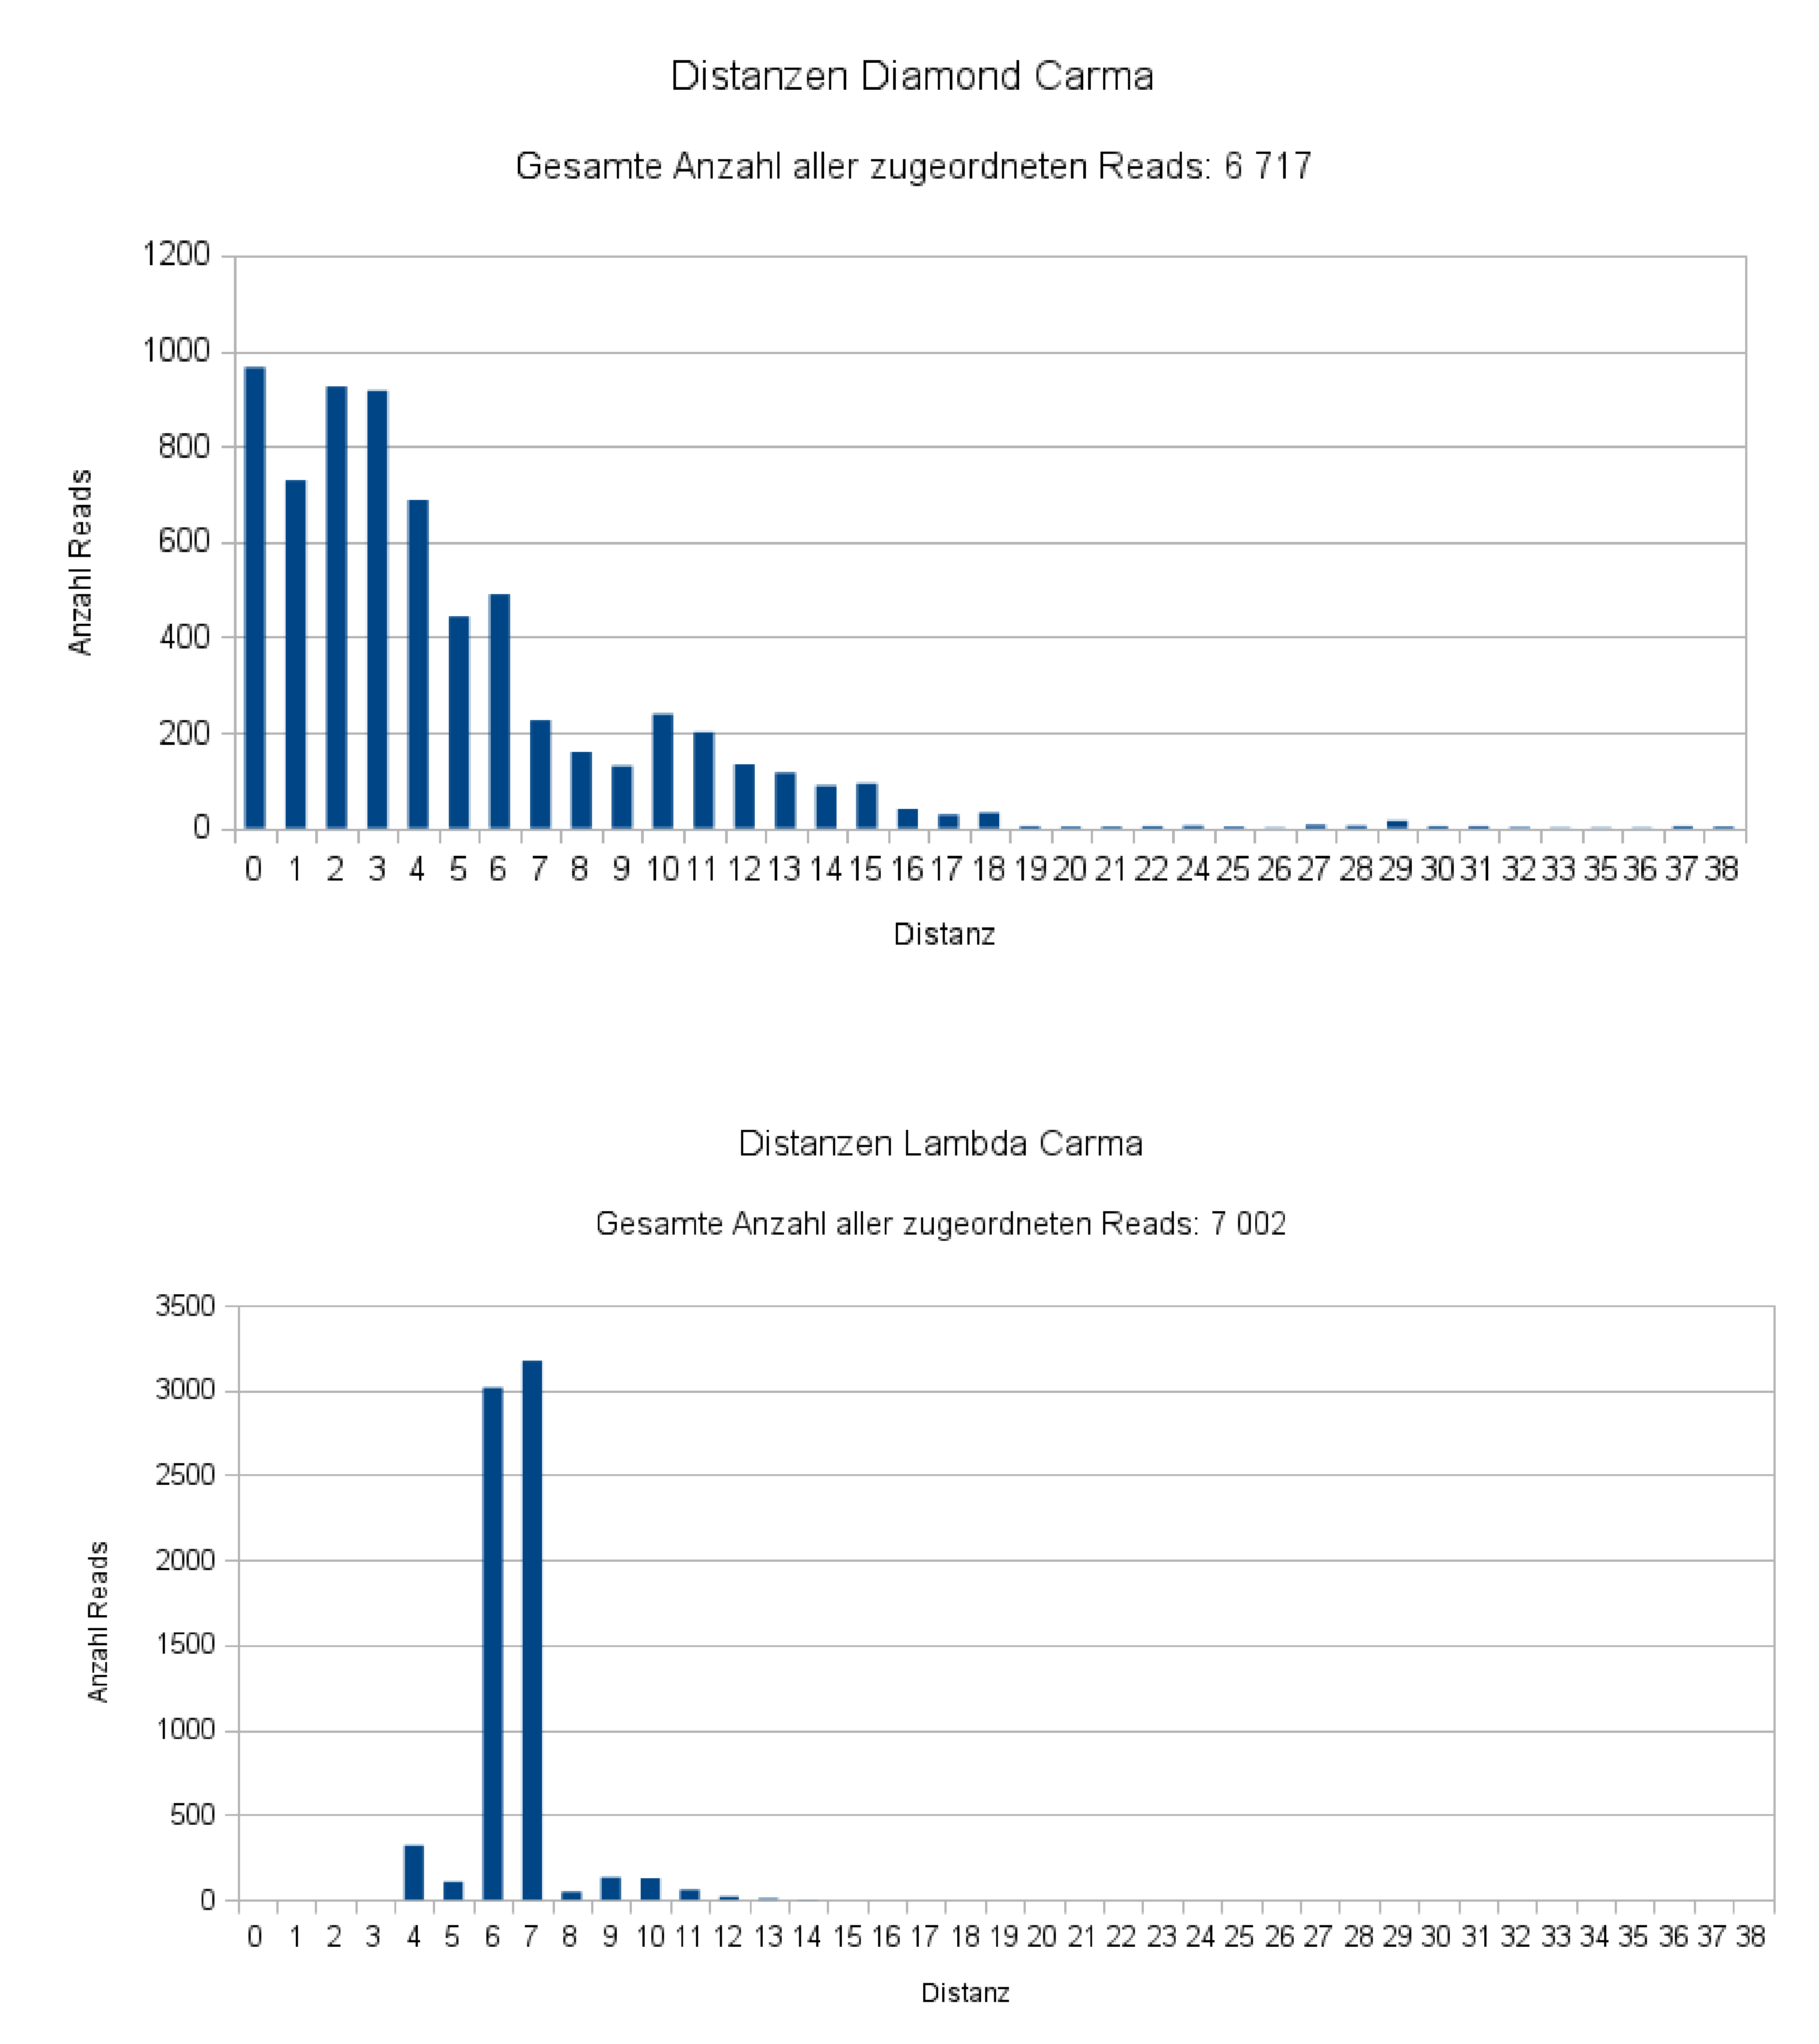
\includegraphics[width=\linewidth,height=13cm,
      keepaspectratio]{Abbildungen/Carma_Distanzen_both.png}
      \caption[Distanzverteilung der Reads: Carma Benchmark-Datensatz.]{\small{Distanzverteilung der Reads: Carma Benchmark-Datensatz.\newline \textbf{Oben}: Ausgabe Diamond. \textbf{Unten}: Ausgabe Lambda.}}
      \label{fig:carma}
      \centering     
    \end{figure}

%FACS Abb. 6.2
    \begin{figure}[H]
      \centering
      \noindent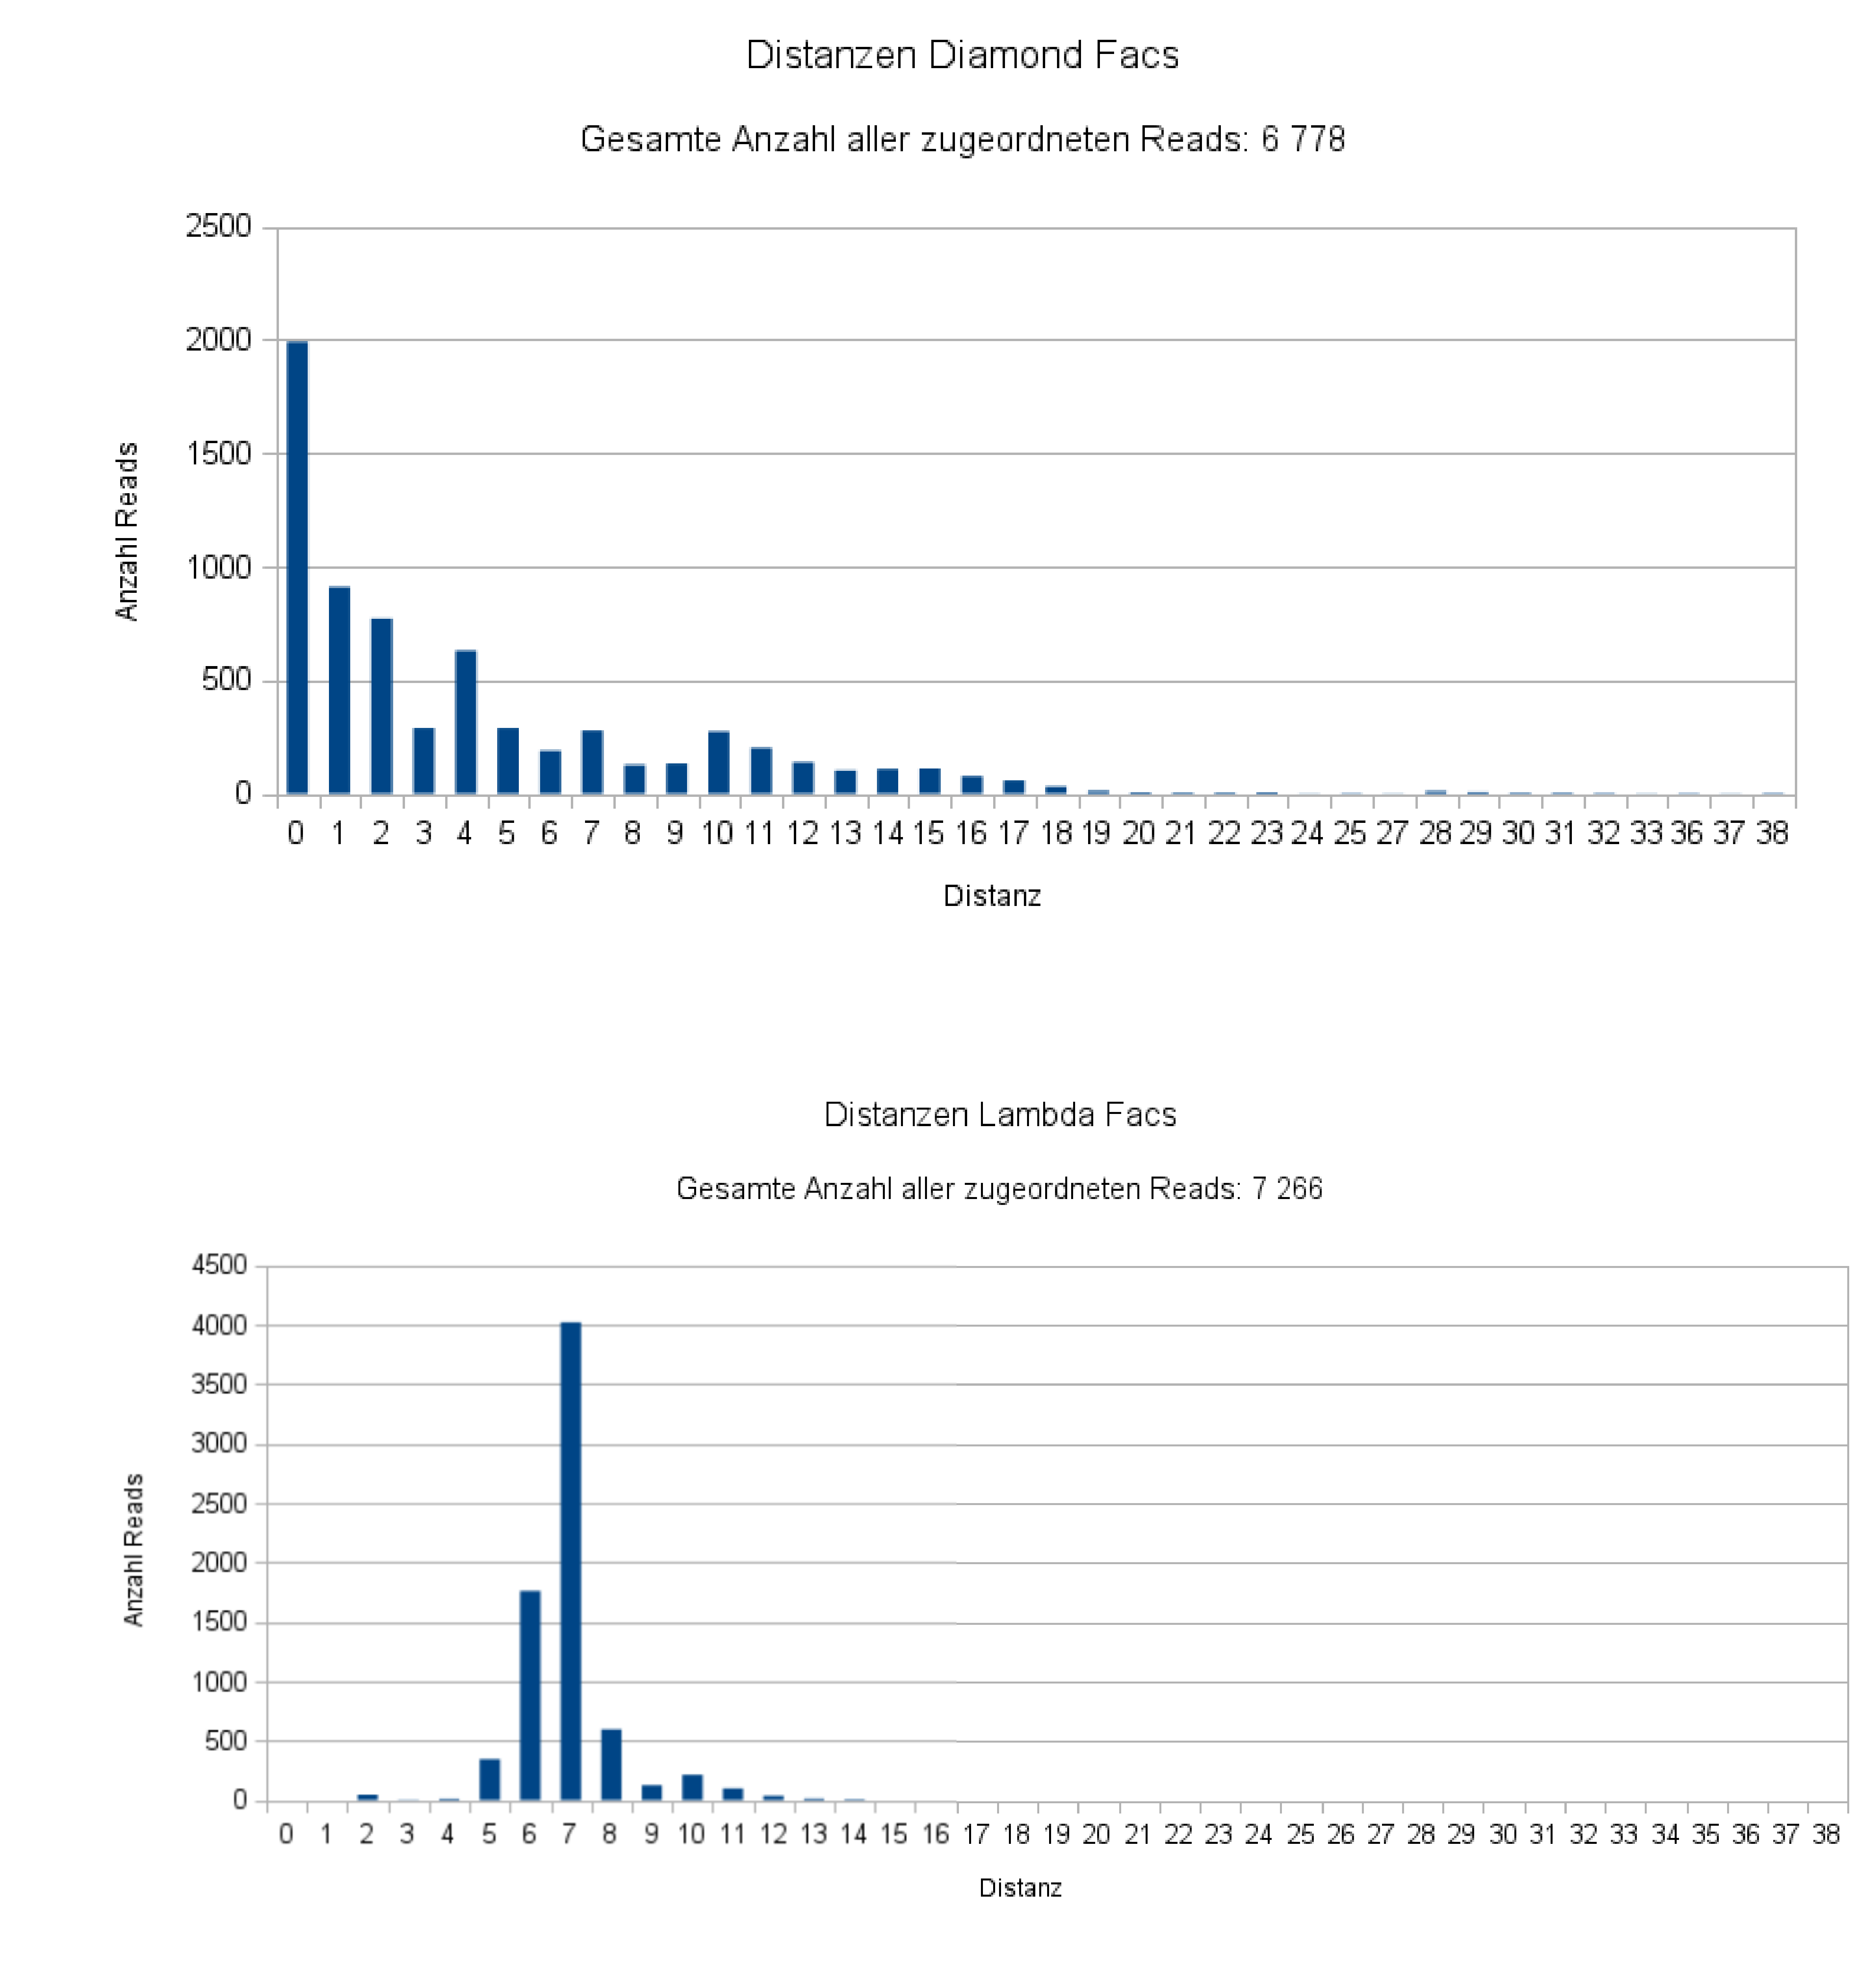
\includegraphics[width=\linewidth,height=13cm,
      keepaspectratio]{Abbildungen/Facs_Distanzen_both.png}
      \caption[Distanzverteilung der Reads: FACS Benchmark-Datensatz.]{\small{Distanzverteilung der Reads: FACS Benchmark-Datensatz.\newline \textbf{Oben}: Ausgabe Diamond. \textbf{Unten}: Ausgabe Lambda.}}
      \label{fig:facs}
    \end{figure}
    
%PhyloPythia Abb. 6.3
     \begin{figure}[H]
      \centering
      \noindent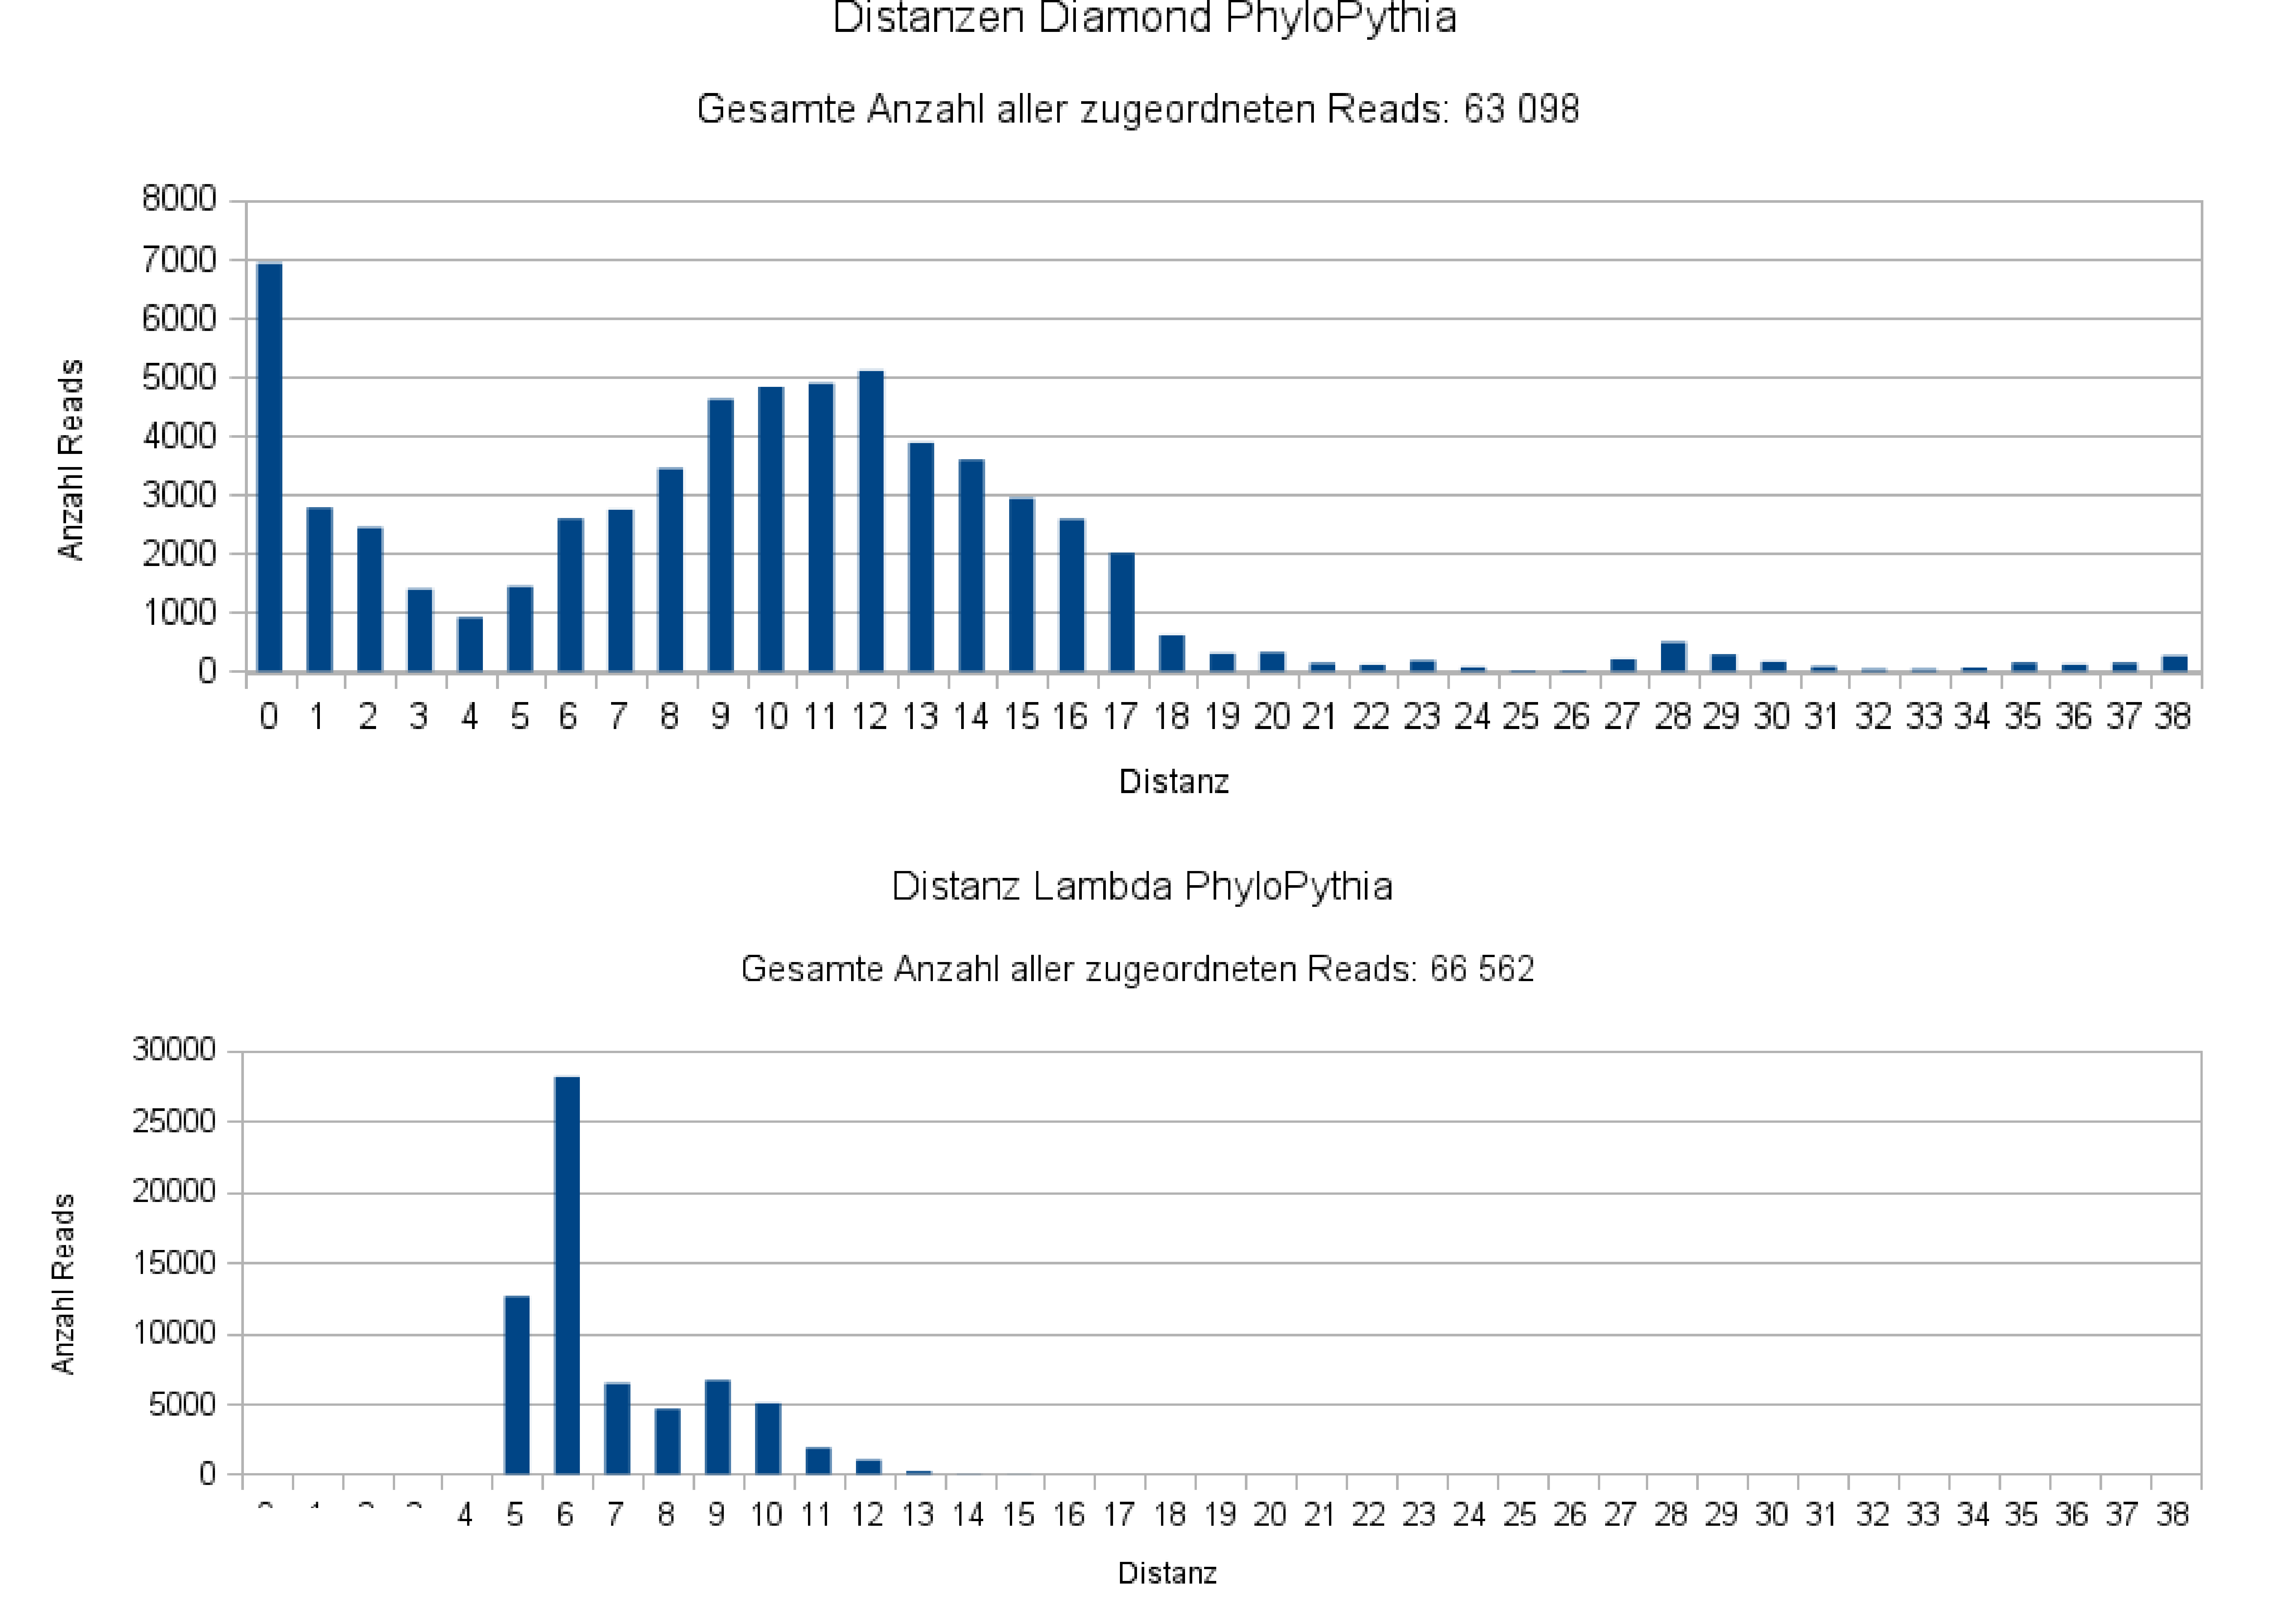
\includegraphics[width=\linewidth,height=20cm,
      keepaspectratio]{Abbildungen/PhyloPythia_Distanzen_both.png}
      \caption[Distanzverteilung der Reads: PhyloPythia Benchmark-Datensatz.]{\small{Distanzverteilung der Reads: PhyloPythia Benchmark-Datensatz.\newline \textbf{Oben}: Ausgabe Diamond. \textbf{Unten}: Ausgabe Lambda.}}
      \label{fig:phylopythia}
    \end{figure}


%Metaphyler Abb. 6.4
\begin{figure}[H]
      \centering
      \noindent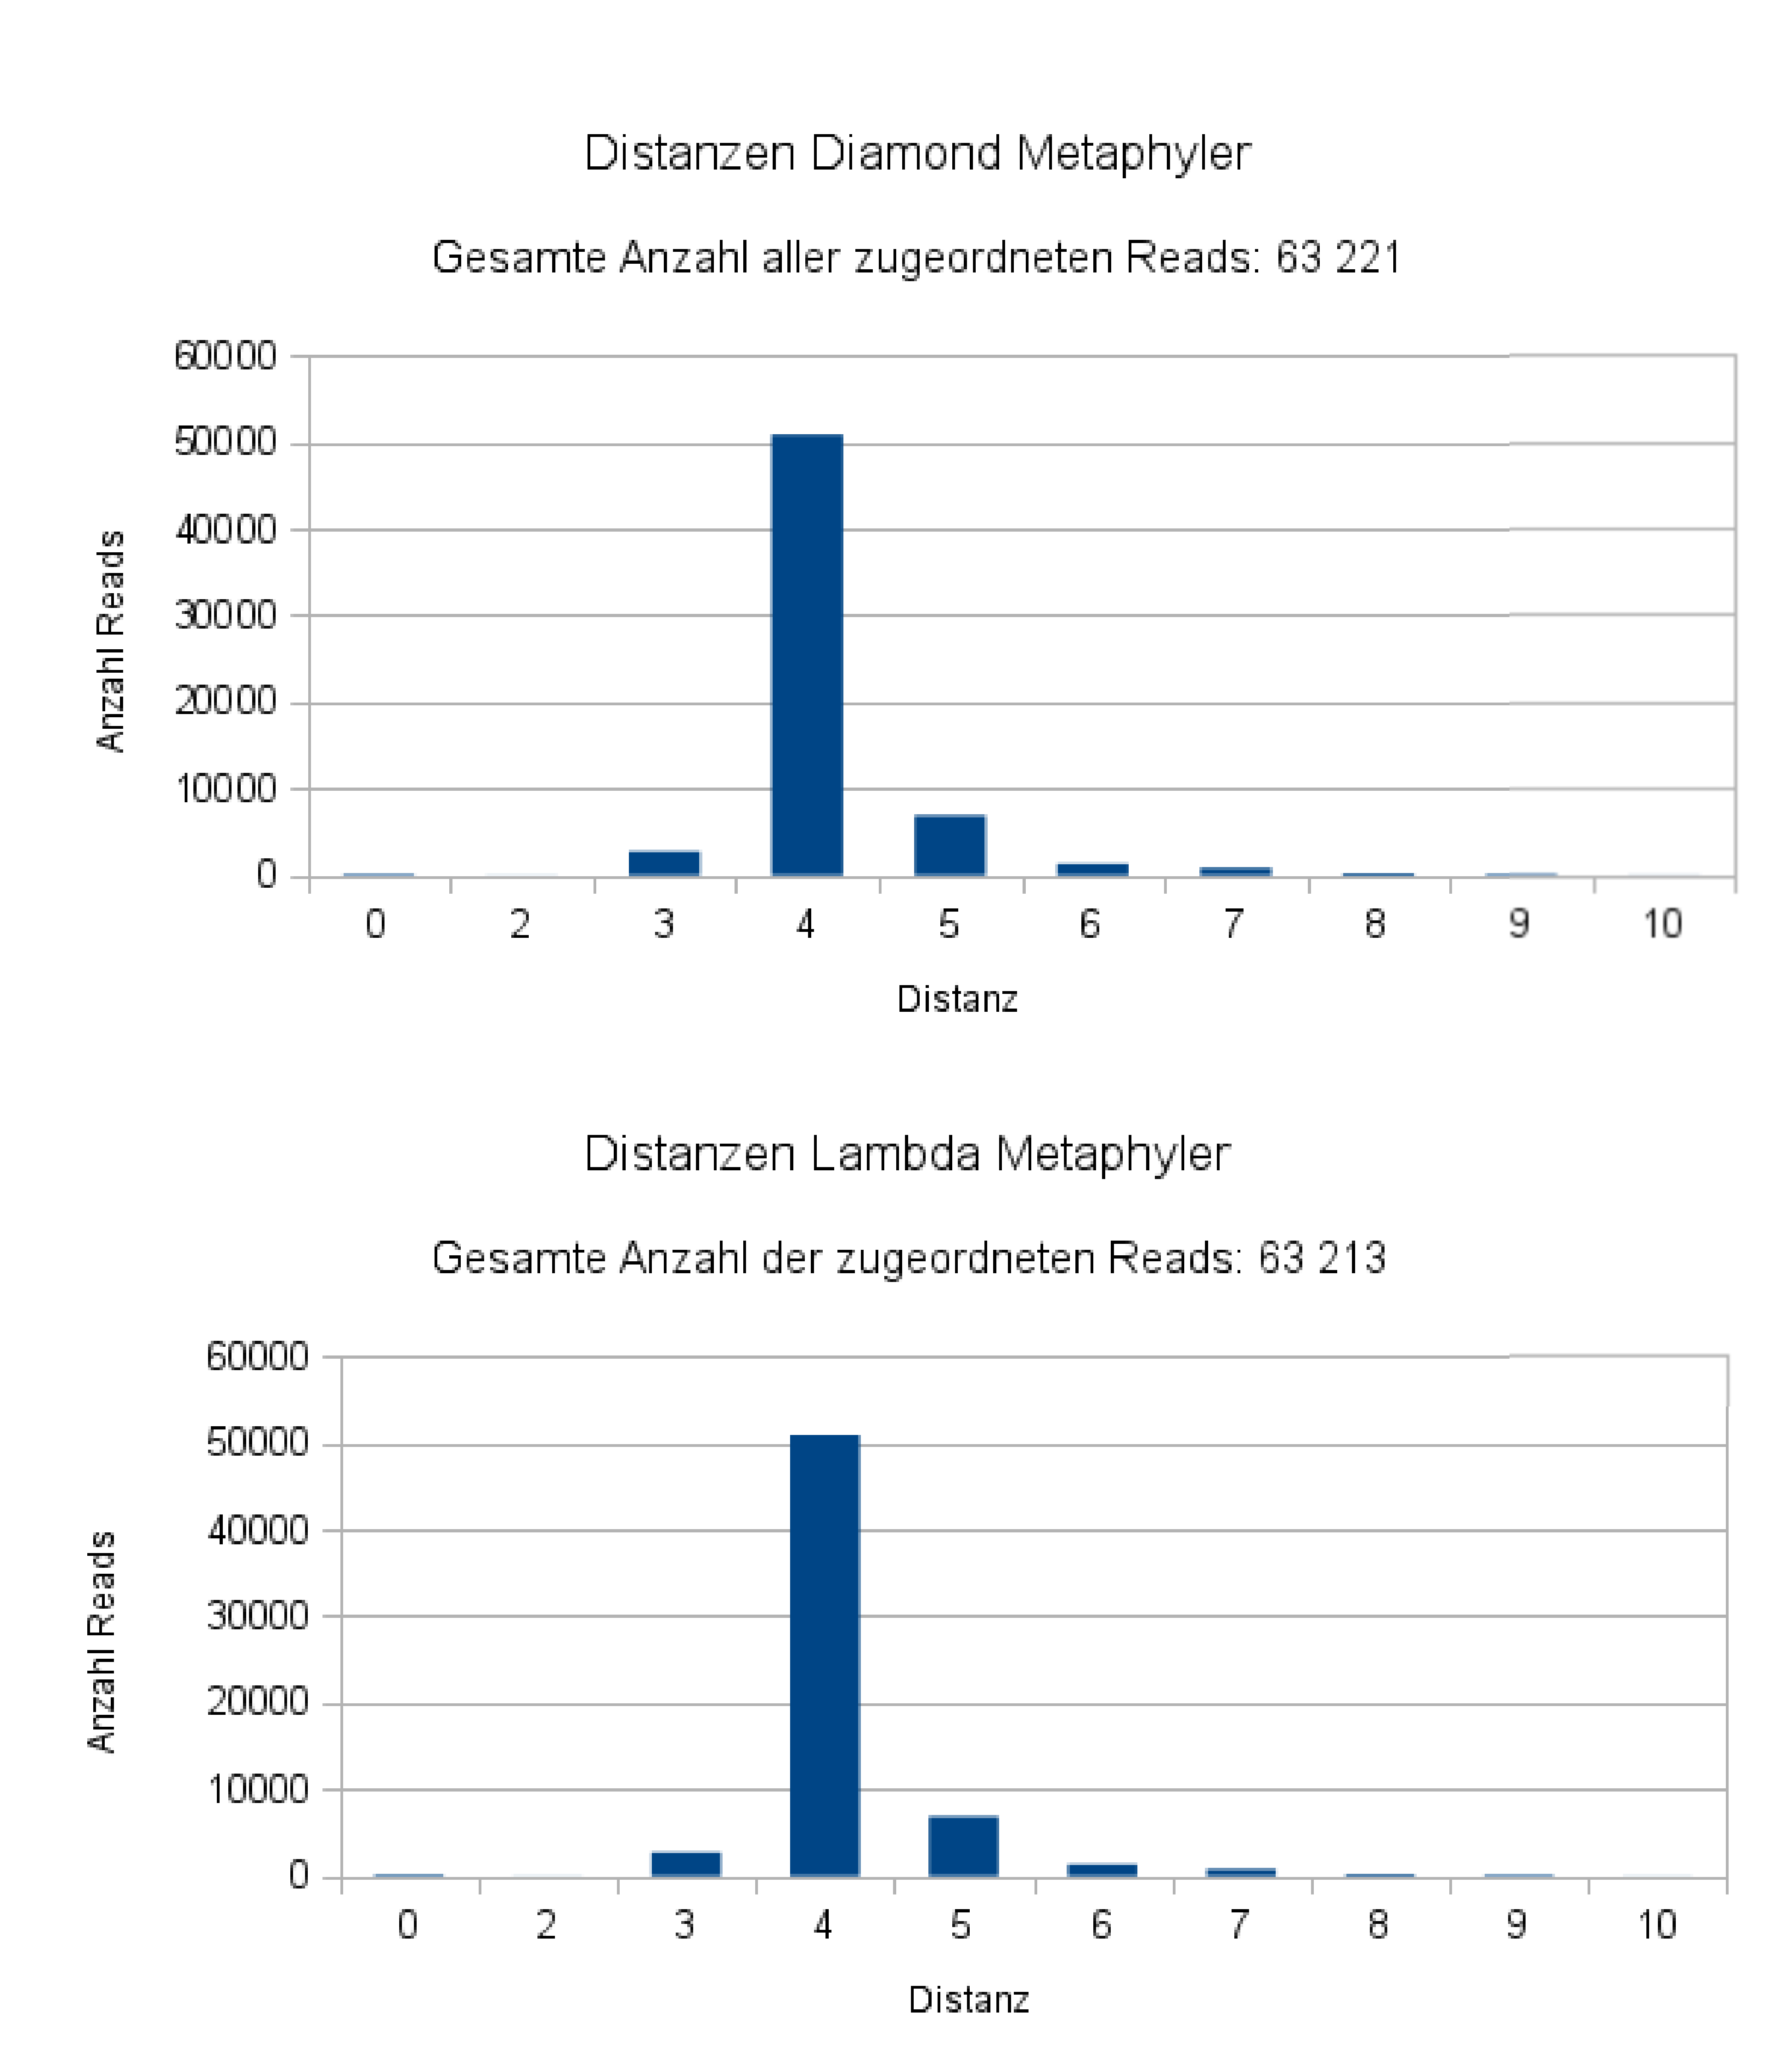
\includegraphics[width=\linewidth,height=15cm,
      keepaspectratio]{Abbildungen/Metaphyler_Distanzen_both.png}
      \caption[Distanzverteilung der Reads: Metaphyler Benchmark-Datensatz.]{\small{Distanzverteilung der Reads: Metaphyler Benchmark-Datensatz.\newline \textbf{Oben}: Ausgabe Diamond. \textbf{Unten}: Ausgabe Lambda.}}
      \label{fig:metaphyler}
    \end{figure}

%PymmBL Abb. 6.5
     \begin{figure}[H]
      \centering
      \noindent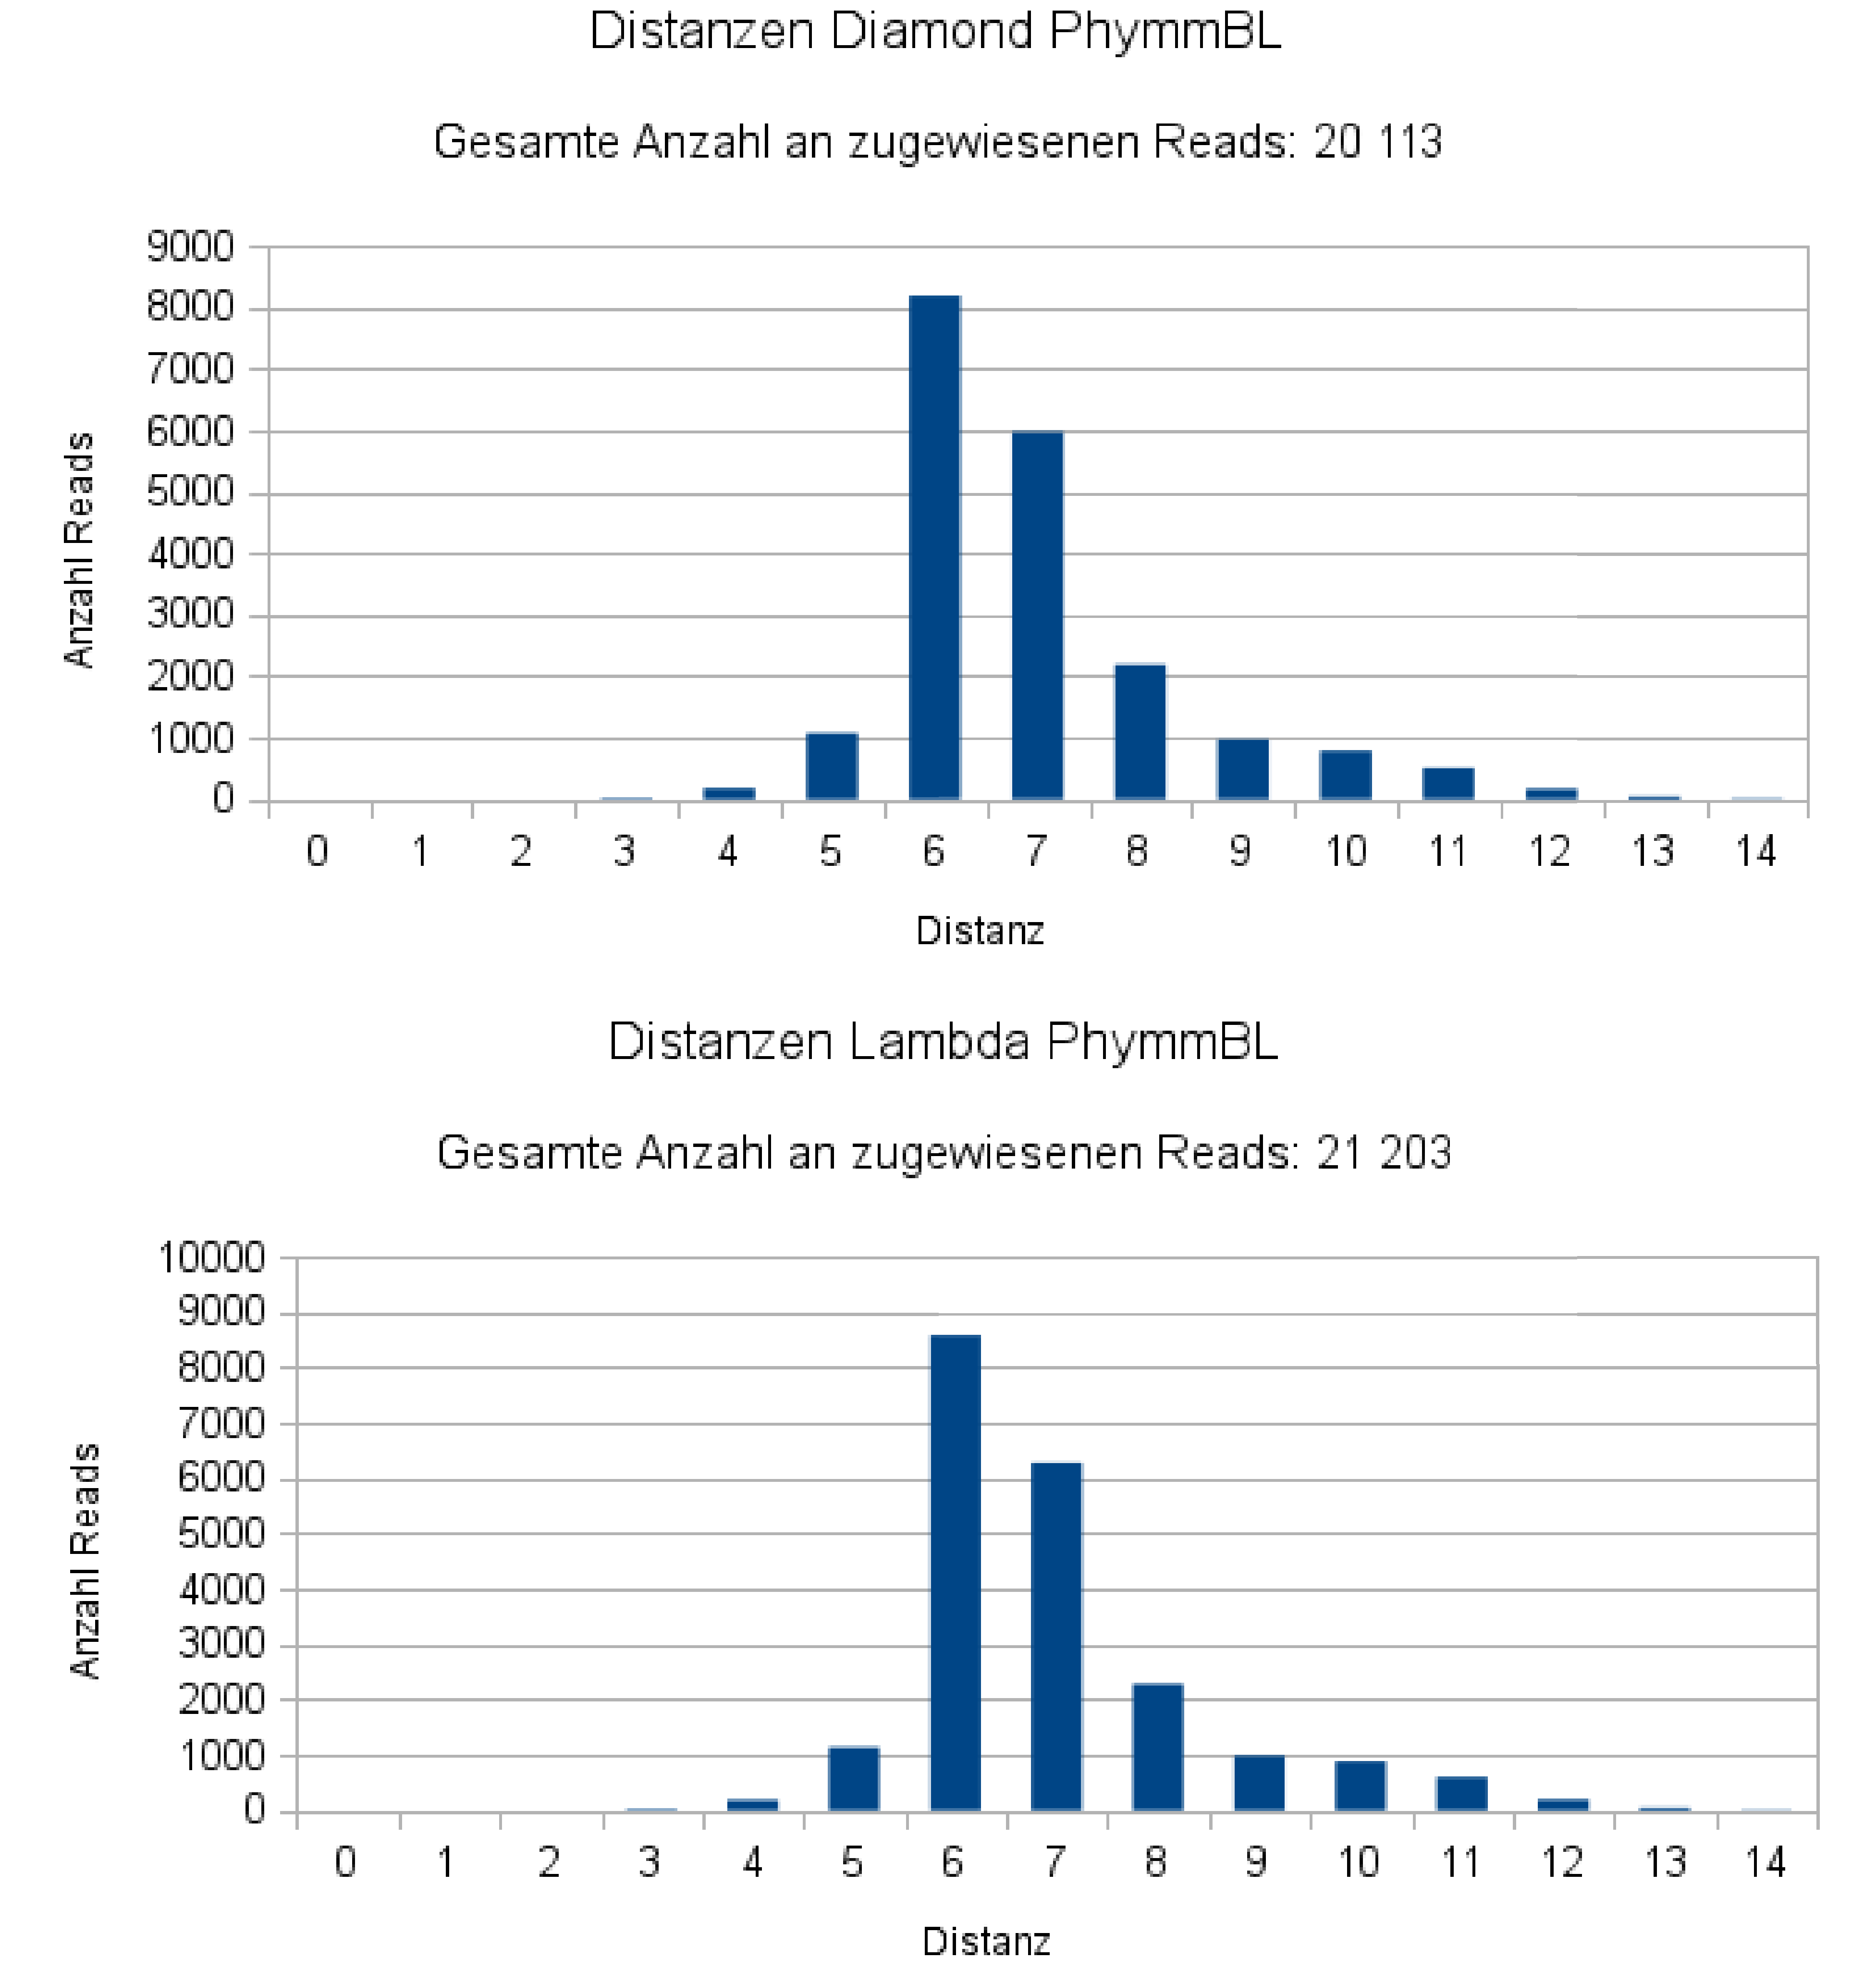
\includegraphics[width=\linewidth,height=15cm,
      keepaspectratio]{Abbildungen/PhymmBL_Distanzen_both.png}
      \caption[Distanzverteilung der Reads: PhymmBL Benchmark-Datensatz.]{\small{Distanzverteilung der Reads: PhymmBL Benchmark-Datensatz.\newline \textbf{Oben}: Ausgabe Diamond. \textbf{Unten}: Ausgabe Lambda.}}
      \label{fig:phymmbl}
    \end{figure}
    
    
    %RAIphy Abb. 6.6
     \begin{figure}[H]
      \centering
      \noindent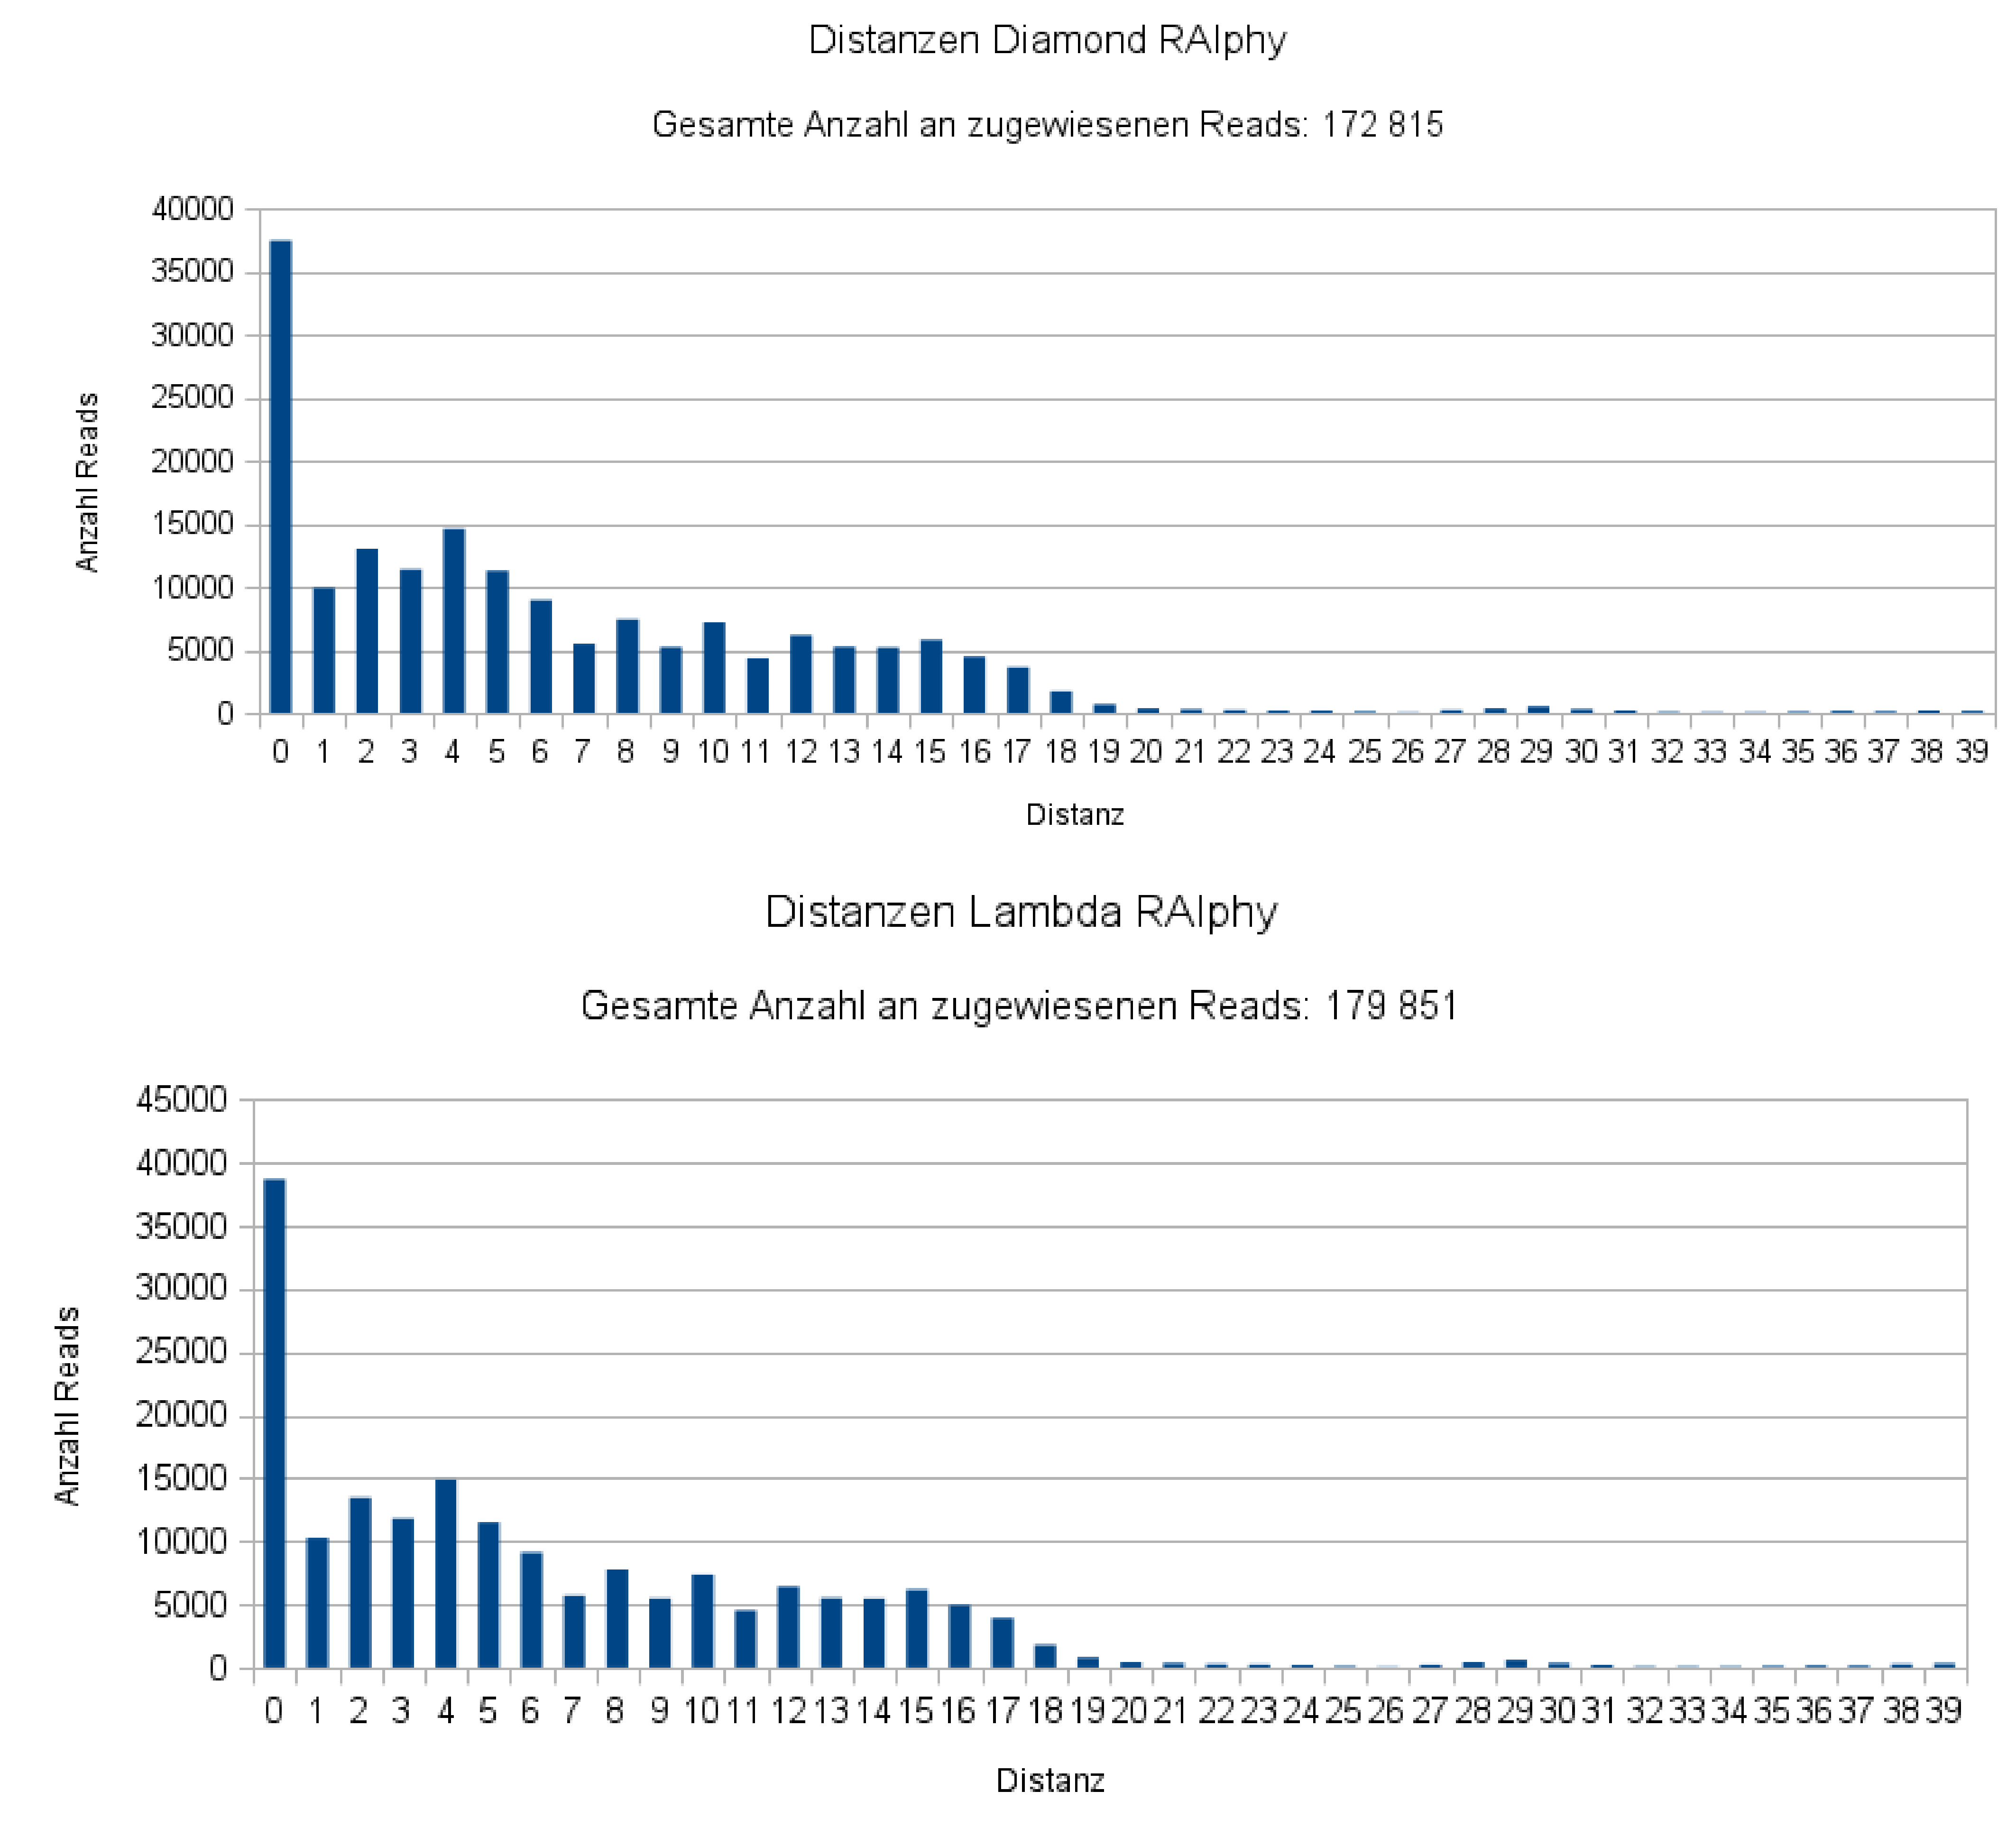
\includegraphics[width=\linewidth,height=15cm,
      keepaspectratio]{Abbildungen/RAIphy_Distanzen_both.png}
      \caption[Distanzverteilung der Reads: RAIphy Benchmark-Datensatz.]{\small{Distanzverteilung der Reads: RAIphy Benchmark-Datensatz.\newline \textbf{Oben}: Ausgabe Diamond. \textbf{Unten}: Ausgabe Lambda.}}
      \label{fig:raiphy}
    \end{figure}

\end{document}




